%%
% The BIThesis Template for Bachelor Graduation Thesis
%
% 北京理工大学毕业设计(论文) —— 使用 XeLaTeX 编译
%
% Copyright 2020 Spencer Woo
%
% This work may be distributed and/or modified under the
% conditions of the LaTeX Project Public License, either version 1.3
% of this license or (at your option) any later version.
% The latest version of this license is in
%   http://www.latex-project.org/lppl.txt
% and version 1.3 or later is part of all distributions of LaTeX
% version 2005/12/01 or later.
%
% This work has the LPPL maintenance status `maintained'.
%
% The Current Maintainer of this work is Spencer Woo.
%
% Compile with: xelatex -> biber -> xelatex -> xelatex

% 章节支持、单面打印:ctexbook
\documentclass[UTF8,AutoFakeBold,AutoFakeSlant,zihao=-4,oneside,openany]{ctexbook}
\usepackage[a4paper,left=3cm,right=2.6cm,top=3.5cm,bottom=2.9cm]{geometry}
% 目前 29mm 最接近 Word 排版
\usepackage{xeCJK}
\usepackage{titletoc}
\usepackage{fontspec}
\usepackage{setspace}
\usepackage{graphicx}
\usepackage{fancyhdr}
\usepackage{pdfpages}
\usepackage{setspace}
\usepackage{booktabs}
\usepackage{multirow}
\usepackage{caption}
\usepackage{tikz}
\usepackage{etoolbox}
\usepackage{hyperref}
\usepackage{xcolor}
\usepackage{caption}
\usepackage{array}
\usepackage{amsmath}
\usepackage{amssymb}
\usepackage{pdfpages}
\usepackage{float}
\usepackage{subfigure}

% 设置参考文献编译后端为 biber,引用格式为 GB/T7714-2015 格式
% 参考文献使用宏包见 https://github.com/hushidong/biblatex-gb7714-2015
\usepackage[
  backend=biber,
  style=gb7714-2015,
  gbalign=gb7714-2015,
  gbnamefmt=lowercase,
  doi=false,
  url=false
]{biblatex}

% 参考文献引用文件位于 misc/ref.bib
\addbibresource{misc/ref.bib}

% 西文字体默认为 Times New Roman
\setromanfont{Times New Roman}
% 论文题目字体为华文细黑
\setCJKfamilyfont{xihei}{STXihei}
\newcommand{\xihei}{\CJKfamily{xihei}}

% 在这里填写你的论文中英文题目
\newcommand{\thesisTitle}{固定翼紧密编队控制及应用}
\newcommand{\thesisTitleEN}{Close Formation Control and Application of Fixed-wing UAV}

% 在这里填写你的相关信息
\newcommand{\deptName}{宇航学院}
\newcommand{\majorName}{飞行器设计与工程}
\newcommand{\yourName}{李\quad 顺}
\newcommand{\yourStudentID}{1120160012}
\newcommand{\mentorName}{王佳楠}

% 主题页面格式:BIThesis
\fancypagestyle{BIThesis}{
  % 页眉高度
  \setlength{\headheight}{20pt}
  % 页码高度(不完美,比规定稍微靠下 2mm)
  \setlength{\footskip}{14pt}

  \fancyhf{}
  % 定义页眉、页码
  \fancyhead[C]{\zihao{4}\ziju{0.08}\songti{北京理工大学本科生毕业设计(论文)}}
  \fancyfoot[C]{\songti\zihao{5} \thepage}
  % 页眉分割线稍微粗一些
  \renewcommand{\headrulewidth}{0.6pt}
}

% 设置章节格式
% 一级标题:黑体,三号,加粗;间距:段前 0.5 行,段后 1 行;
\ctexset{chapter={
    name = {第,章},
    number = {\arabic{chapter}},
    format = {\heiti \bfseries \centering \zihao{3}},
    aftername = \hspace{9bp},
    pagestyle = BIThesis,
    beforeskip = 8bp,
    afterskip = 32bp,
    fixskip = true,
  }
}

% 二级标题:黑体,四号,加粗;间距:段前 0.5 行,段后 0 行;
\ctexset{section={
    number = {\thechapter.\hspace{4bp}\arabic{section}},
    format = {\heiti \raggedright \bfseries \zihao{4}},
    aftername = \hspace{8bp},
    beforeskip = 20bp plus 1ex minus .2ex,
    afterskip = 18bp plus .2ex,
    fixskip = true,
  }
}

% 三级标题:黑体、小四、加粗;间距:段前 0.5 行,段后 0 行;
\ctexset{subsection={
    number = {\thechapter.\hspace{3bp}\arabic{section}.\hspace{3bp}\arabic{subsection}},
    format = {\heiti \bfseries \raggedright \zihao{-4}},
    aftername = \hspace{7bp},
    beforeskip = 17bp plus 1ex minus .2ex,
    afterskip = 14bp plus .2ex,
    fixskip = true,
  }
}

% 设置目录样式
% 添加 PDF 链接
\addtocontents{toc}{\protect\hypersetup{hidelinks}}

% 解决「目录」二字的格式问题
\renewcommand{\contentsname}{
  \fontsize{16pt}{\baselineskip}
  \normalfont\heiti{目~~~~录}
  \vspace{-8pt}
}
% 定义目录样式
\titlecontents{chapter}[0pt]{\songti \zihao{-4}}
{\thecontentslabel\hspace{\ccwd}}{}
{\hspace{.5em}\titlerule*{.}\contentspage}
\titlecontents{section}[2\ccwd]{\songti \zihao{-4}}
{\thecontentslabel\hspace{\ccwd}}{}
{\hspace{.5em}\titlerule*{.}\contentspage}
\titlecontents{subsection}[4\ccwd]{\songti \zihao{-4}}
{\thecontentslabel\hspace{\ccwd}}{}
{\hspace{.5em}\titlerule*{.}\contentspage}

% 前置页面(原创性声明、中英文摘要、目录等)
\renewcommand{\frontmatter}{
  \pagenumbering{Roman}
  \pagestyle{BIThesis}
}

% 正文页面
\renewcommand{\mainmatter}{
  \pagenumbering{arabic}
  \pagestyle{BIThesis}
}

% 设置 caption 与 figure 之间的距离
\setlength{\abovecaptionskip}{11pt}
\setlength{\belowcaptionskip}{9pt}

% 设置图片的 caption 格式
\renewcommand{\thefigure}{\thechapter-\arabic{figure}}
\captionsetup[figure]{font=small,labelsep=space}

% 设置表格的 caption 与 table 之间的垂直距离
\captionsetup[table]{skip=2pt}

% 设置表格的 caption 格式
\renewcommand{\thetable}{\thechapter-\arabic{table}}
\captionsetup[table]{font=small,labelsep=space}

% 设置数学公式编号格式
\renewcommand{\theequation}{\arabic{chapter}-\arabic{equation}}

% 文档开始
\begin{document}

% 标题页面:如无特殊需要,本部分无需改动
%%
% The BIThesis Template for Bachelor Graduation Thesis
%
% 北京理工大学毕业设计(论文)封面页 —— 使用 XeLaTeX 编译
%
% Copyright 2020 Spencer Woo
%
% This work may be distributed and/or modified under the
% conditions of the LaTeX Project Public License, either version 1.3
% of this license or (at your option) any later version.
% The latest version of this license is in
%   http://www.latex-project.org/lppl.txt
% and version 1.3 or later is part of all distributions of LaTeX
% version 2005/12/01 or later.
%
% This work has the LPPL maintenance status `maintained'.
%
% The Current Maintainer of this work is Spencer Woo.
%
% 封面
%
% 如无特殊需要,本页面无需更改

% Underline new command for student information
% Usage: \dunderline[<offset>]{<line_thickness>}
\newcommand\dunderline[3][-1pt]{{%
  \setbox0=\hbox{#3}
  \ooalign{\copy0\cr\rule[\dimexpr#1-#2\relax]{\wd0}{#2}}}}

% Cover Page
\begin{titlepage}
  \vspace*{19mm}
  \centering

  
\includegraphics[width=9.87cm]{images/header.png}

  \vspace*{-3mm}

  \zihao{-0}\textbf{\ziju{0.12}\songti{本科生毕业设计(论文)}}

  \vspace{16mm}

  \zihao{2}\textbf{\xihei\thesisTitle}

  \vspace{3mm}

  \begin{spacing}{1.2}
    \zihao{3}\selectfont{\textbf{\thesisTitleEN}}
  \end{spacing}

  \vspace{15mm}

  \flushleft
  \begin{spacing}{1.8}
    \hspace{27mm}\songti\zihao{3}\selectfont{学\hspace{11mm}院:\dunderline[-10pt]{1pt}{\makebox[78mm][c]{\deptName}}}

    \hspace{27mm}\songti\zihao{3}\selectfont{专\hspace{11mm}业:\dunderline[-10pt]{1pt}{\makebox[78mm][c]{\majorName}}}

    \hspace{27mm}\songti\zihao{3}\selectfont{学生姓名:\dunderline[-10pt]{1pt}{\makebox[78mm][c]{\yourName}}}

    \hspace{27mm}\songti\zihao{3}\selectfont{学\hspace{11mm}号:\dunderline[-10pt]{1pt}{\makebox[78mm][c]{\yourStudentID}}}

    \hspace{27mm}\songti\zihao{3}\selectfont{指导教师:\dunderline[-10pt]{1pt}{\makebox[78mm][c]{\mentorName}}}
  \end{spacing}

  \vspace{25mm}

  \centering
  \zihao{3}\ziju{0.5}\songti{\today}
\end{titlepage}


% 前置页面定义
\frontmatter
% 原创性声明:如无特殊需要,本部分无需改动
% 更改为 PDF 页面插入,如需要添加内容,可考虑先用 Word 制作再覆盖 misc/1_originality.pdf

\includepdf{misc/1_originality.pdf}
\newpage
%%%
% The BIThesis Template for Bachelor Graduation Thesis
%
% 北京理工大学毕业设计(论文)原创性声明页 —— 使用 XeLaTeX 编译
%
% Copyright 2020 Spencer Woo
%
% This work may be distributed and/or modified under the
% conditions of the LaTeX Project Public License, either version 1.3
% of this license or (at your option) any later version.
% The latest version of this license is in
%   http://www.latex-project.org/lppl.txt
% and version 1.3 or later is part of all distributions of LaTeX
% version 2005/12/01 or later.
%
% This work has the LPPL maintenance status `maintained'.
%
% The Current Maintainer of this work is Spencer Woo.
%
% 如无特殊需要,本页面无需更改

% 原创性声明页无页码页面格式
\fancypagestyle{originality}{
  % 页眉高度
  \setlength{\headheight}{20pt}

  % 页眉和页脚(页码)的格式设定
  \fancyhf{}
  \fancyhead[C]{\zihao{4}\ziju{0.08}\songti{北京理工大学本科生毕业设计(论文)}}

  % 页眉分割线稍微粗一些
  \renewcommand{\headrulewidth}{0.6pt}
}

\pagestyle{originality}
\topskip=0pt

% 圆形数字编号定义
\newcommand{\circled}[2][]{\tikz[baseline=(char.base)]
  {\node[shape = circle, draw, inner sep = 1pt]
  (char) {\phantom{\ifblank{#1}{#2}{#1}}};
  \node at (char.center) {\makebox[0pt][c]{#2}};}}
\robustify{\circled}

% 设置行间距
\setlength{\parskip}{0.4em}
\renewcommand{\baselinestretch}{1.41}

% 顶部空白
\vspace*{-6mm}

% 原创性声明部分
\begin{center}
  \heiti\zihao{2}\textbf{原创性声明}
\end{center}

% 本部分字号为小三
\zihao{-3}

本人郑重声明:所呈交的毕业设计(论文),是本人在指导老师的指导下独立进行研究所取得的成果。除文中已经注明引用的内容外,本文不包含任何其他个人或集体已经发表或撰写过的研究成果。对本文的研究做出重要贡献的个人和集体,均已在文中以明确方式标明。

特此申明。

\vspace{13mm}

\begin{flushright}
  本人签名:\hspace{40mm}日\hspace{2.5mm}期:\hspace{13mm}年\hspace{8mm}月\hspace{8mm}日
\end{flushright}

\vspace{17mm}

% 使用授权声明部分
\begin{center}
  \heiti\zihao{2}\textbf{关于使用授权的声明}
\end{center}

本人完全了解北京理工大学有关保管、使用毕业设计(论文)的规定,其中包括:\circled{1}学校有权保管、并向有关部门送交本毕业设计(论文)的原件与复印件;\circled{2}学校可以采用影印、缩印或其它复制手段复制并保存本毕业设计(论文);\circled{3}学校可允许本毕业设计(论文)被查阅或借阅;\circled{4}学校可以学术交流为目的,复制赠送和交换本毕业设计(论文);\circled{5}学校可以公布本毕业设计(论文)的全部或部分内容。

\vspace*{1mm}

\begin{flushright}
  \begin{spacing}{1.65}
    \zihao{-3}
    本人签名:\hspace{40mm}日\hspace{2.5mm}期:\hspace{13mm}年\hspace{8mm}月\hspace{8mm}日\\
    指导老师签名:\hspace{40mm}日\hspace{2.5mm}期:\hspace{13mm}年\hspace{8mm}月\hspace{8mm}日
  \end{spacing}
\end{flushright}

\newpage

% 摘要:在摘要相应的 TeX 文件处进行摘要部分的撰写
%%
% The BIThesis Template for Bachelor Graduation Thesis
%
% 北京理工大学毕业设计(论文)中英文摘要 —— 使用 XeLaTeX 编译
%
% Copyright 2020 Spencer Woo
%
% This work may be distributed and/or modified under the
% conditions of the LaTeX Project Public License, either version 1.3
% of this license or (at your option) any later version.
% The latest version of this license is in
%   http://www.latex-project.org/lppl.txt
% and version 1.3 or later is part of all distributions of LaTeX
% version 2005/12/01 or later.
%
% This work has the LPPL maintenance status `maintained'.
%
% The Current Maintainer of this work is Spencer Woo.

% 中英文摘要章节
\topskip=0pt
\zihao{-4}

\vspace*{-7mm}

\begin{center}
  \heiti\zihao{-2}\textbf{\thesisTitle}
\end{center}

\vspace*{2mm}

\addcontentsline{toc}{chapter}{摘~~~~要}
{\let\clearpage\relax \chapter*{\textmd{摘~~~~要}}}
\setcounter{page}{1}

\vspace*{1mm}

\setstretch{1.53}
\setlength{\parskip}{0em}

% 中文摘要正文从这里开始
本文……。

\textcolor{blue}{摘要正文选用模板中的样式所定义的“正文”,每段落首行缩进 2 个字符;或者手动设置成每段落首行缩进 2 个汉字,字体:宋体,字号:小四,行距:固定值 22 磅,间距:段前、段后均为 0 行。阅后删除此段。}

\textcolor{blue}{摘要是一篇具有独立性和完整性的短文,应概括而扼要地反映出本论文的主要内容。包括研究目的、研究方法、研究结果和结论等,特别要突出研究结果和结论。中文摘要力求语言精炼准确,本科生毕业设计(论文)摘要建议 300-500 字。摘要中不可出现参考文献、图、表、化学结构式、非公知公用的符号和术语。英文摘要与中文摘要的内容应一致。阅后删除此段。}

\vspace{4ex}\noindent\textbf{\heiti 关键词:北京理工大学;本科生;毕业设计(论文)}
\newpage

% 英文摘要章节
\topskip=0pt

\vspace*{2mm}

\begin{spacing}{0.95}
  \centering
  \heiti\zihao{3}\textbf{\thesisTitleEN}
\end{spacing}

\vspace*{17mm}

\addcontentsline{toc}{chapter}{Abstract}
{\let\clearpage\relax \chapter*{
  \zihao{-3}\textmd{Abstract}\vskip -3bp}}
\setcounter{page}{2}

\setstretch{1.53}
\setlength{\parskip}{0em}

% 英文摘要正文从这里开始
In order to study……

\textcolor{blue}{Abstract 正文设置成每段落首行缩进 2 字符,字体:Times New Roman,字号:小四,行距:固定值 22 磅,间距:段前、段后均为 0 行。阅后删除此段。}

\vspace{3ex}\noindent\textbf{Key Words: BIT; Undergraduate; Graduation Project (Thesis)}
\newpage

% 目录:如无特殊需要,本部分无需改动
%%
% The BIThesis Template for Bachelor Graduation Thesis
%
% 北京理工大学毕业设计(论文)目录 —— 使用 XeLaTeX 编译
%
% Copyright 2020 Spencer Woo
%
% This work may be distributed and/or modified under the
% conditions of the LaTeX Project Public License, either version 1.3
% of this license or (at your option) any later version.
% The latest version of this license is in
%   http://www.latex-project.org/lppl.txt
% and version 1.3 or later is part of all distributions of LaTeX
% version 2005/12/01 or later.
%
% This work has the LPPL maintenance status `maintained'.
%
% The Current Maintainer of this work is Spencer Woo.
%
% 如无特殊需要,本页面无需更改

% 目录开始

% 调整目录行间距
\renewcommand{\baselinestretch}{1.35}
% 目录
\tableofcontents
\newpage


% 正文开始
\mainmatter
% 正文 22 磅的行距
\setlength{\parskip}{0em}
\renewcommand{\baselinestretch}{1.53}

% 第一章
%%
% The BIThesis Template for Bachelor Graduation Thesis
%
% 北京理工大学毕业设计(论文)第一章节 —— 使用 XeLaTeX 编译
%
% Copyright 2020 Spencer Woo
%
% This work may be distributed and/or modified under the
% conditions of the LaTeX Project Public License, either version 1.3
% of this license or (at your option) any later version.
% The latest version of this license is in
%   http://www.latex-project.org/lppl.txt
% and version 1.3 or later is part of all distributions of LaTeX
% version 2005/12/01 or later.
%
% This work has the LPPL maintenance status `maintained'.
%
% The Current Maintainer of this work is Spencer Woo.
%
% 第一章节

\chapter{一级题目}

\section{二级题目}
% 这里插入一个参考文献,仅作参考
正文……\cite{yuFeiJiZongTiDuoXueKeSheJiYouHuaDeXianZhuangYuFaZhanFangXiang2008}

\subsection{三级题目}

正文……\cite{simonyanVeryDeepConvolutional2015}

\textcolor{blue}{正文部分:宋体、小四;正文行距:22磅;间距段前段后均为0行。阅后删除此段。}

\textcolor{blue}{图、表居中,图注标在图下方,表头标在表上方,宋体、五号、居中,1.25倍行距,间距段前段后均为0行,图表与上下文之间各空一行。阅后删除此段。}

\textcolor{blue}{\underline{\underline{图-示例:(阅后删除此段)}}}

\begin{figure}[htbp]
  \vspace{13pt} % 调整图片与上文的垂直距离
  \centering
  
\includegraphics[]{images/bit_logo.png}
  \caption{标题序号}\label{标题序号} % label 用来在文中索引
\end{figure}

\textcolor{blue}{\underline{\underline{表-示例:(阅后删除此段)}}}

\begin{table}[htbp]
  \linespread{1.5}
  \zihao{5}
  \centering
  \caption{统计表}\label{统计表}
  \begin{tabular}{*{5}{>{\centering\arraybackslash}p{2cm}}}
    \hline
    项目    & 产量    & 销量    & 产值   & 比重    \\ \hline
    手机    & 1000  & 10000 & 500  & 50\%  \\
    计算机   & 5500  & 5000  & 220  & 22\%  \\
    笔记本电脑 & 1100  & 1000  & 280  & 28\%  \\ \hline
    合计    & 17600 & 16000 & 1000 & 100\% \\ \hline
    \end{tabular}
\end{table}

\textcolor{blue}{公式标注应于该公式所在行的最右侧。对于较长的公式只可在符号处(+、-、*、/、$\leqslant$ $\geqslant$ 等)转行。在文中引用公式时,在标号前加“式”,如式(1-2)。阅后删除此
段。}

\textcolor{blue}{公式-示例:(阅后删除此段)}

\begin{equation}
    LRI=1\ ∕\ \sqrt{1+{\left(\frac{{\mu }_{R}}{{\mu }_{s}}\right)}^{2}{\left(\frac{{\delta }_{R}}{{\delta }_{s}}\right)}^{2}}
\end{equation}

% 在这里添加第二章、第三章……TeX 文件的引用
\chapter{无人机动力学模型的建立}
\label{chap:formation_dynamic_equ}
本章基于无人机编队的领从方法(leader-follower method)建立无人机编队的相对运动方程。为了与无人机的解耦控制方法相匹配,本文将无人机
运动分为水平平面运动以及竖直平面运动
内分别建立数学模型。由于无人机尺寸小,强度大,飞行包线较小,现做如下假设:
\begin{itemize}
    \item 无人机为具有6自由度的三维空间运动刚体。
    \item 忽略地球自转,将地球作为惯性系。
    \item 忽略地球曲率,即所谓的“平板地球假设”。%TODO:考虑是否要加入大气的假设,以及引用文献
    \item 由于内环控制率以无人机协调(倾斜)转弯(STT)为基础(详见第\ref{chap:hardware}章),飞机满足无侧滑条件,侧滑角为0;即空速方向与机体系$O_bx_b$在同一竖直平面内。
    \item 由于编队飞行时的区域较小,领机与从机的大气环境以及地球重力场等因素完全一致。
\end{itemize}
本章中涉及的坐标系有:
\begin{enumerate}
    \item 地面坐标系$O_gx_gy_gz_g$:$O_g$点选为无人机解锁时的位置,$O_gx_g$轴指向北,$O_gy_g$轴指向东,$O_gz_g$轴符合右手定则,指向下。
    \item 导航坐标系$NED(north-east-down)$:原点选做飞机质心,$N$轴指向北,$E$轴指向东,$D$轴符合右手定则,指向下。
    \item 航迹坐标系$O_kx_ky_kz_k$:$O_k$选为无人机质心,$O_kx_k$轴始终与无人机地速方向一致,$O_kz_k$轴位于包含$O_kx_k$轴的竖直平面内,
    $o_ky_k$符合右手定则,指向右。
    \item 机体坐标系$O_bx_by_bz_b$:$O_b$选为无人机质心,$O_bx_b$位于无人机的对称平面内,平行于机身轴线或者机翼的平均气动弦线,指向前;$O_bz_b$亦在对称平面之内,
    垂直于$O_bx_b$轴,指向下;$O_by_b$垂直于对称平面,指向右。机体坐标系始终与无人机固连。
    \item 气流坐标系$O_ax_ay_az_a$:气流坐标系又被称作风坐标系或者速度坐标系;$O_a$取作无人机质心,$O_ax_a$始终指向无人机的空速方向;$O_az_a$位于无人机对称面之内,
    垂直于$O_ax_a$轴,指向下;$O_ay_a$轴垂直于$O_ax_az_a$平面,指向右。只有在大气风速$V_{wind}=0$时,航迹系的$O_kx_k$才与气流坐标系的$O_ax_a$重合。
\end{enumerate}
本章中领机与从机的各运动学量以及几何关系分别用上标$l,f$标记,从机期望值以$“des”$上标标记;
运动学量以及几何关系所属坐标系关系则用各个坐标系的字母作为下标标记。
领机、从机在水平以及竖直平面内的几何关系分别在图\ref{fig:c02-2d_level_motion}和图\ref{fig:c02-2d_vert_motion}给出;
\begin{figure}[H]
    \centering
    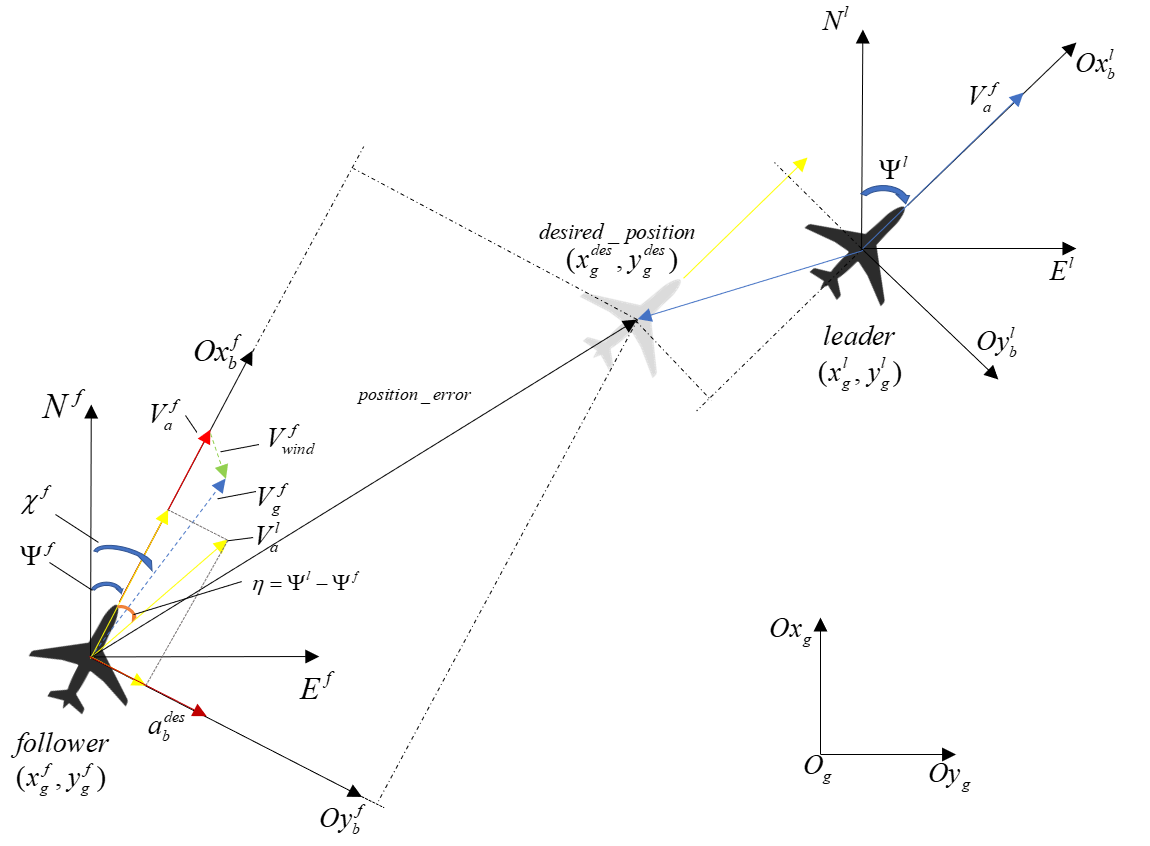
\includegraphics[width=0.75\textwidth]{figures/c2/2d_level_motion.png}
    \caption{水平平面双机编队几何关系}\label{fig:c02-2d_level_motion}
\end{figure}
\begin{figure}[H]
    \centering
    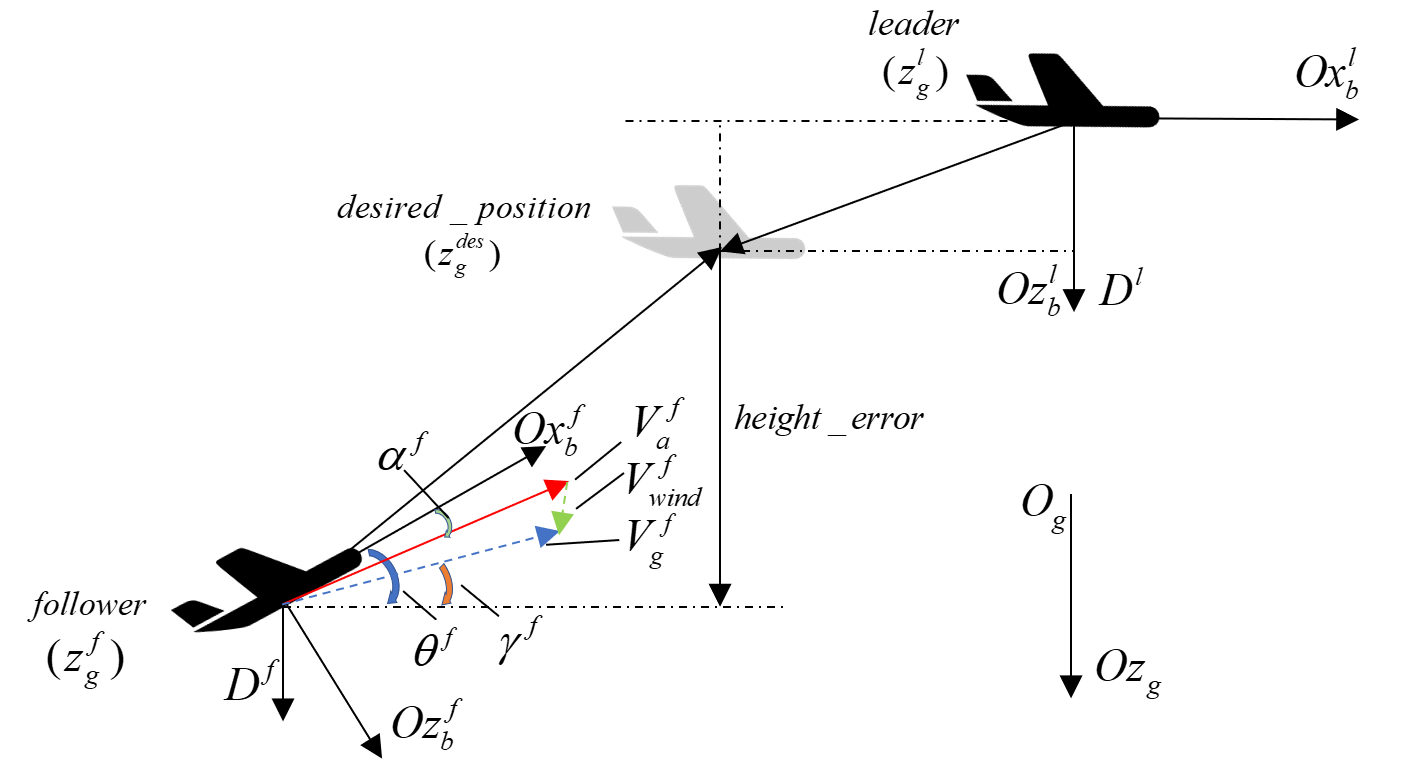
\includegraphics[width=0.75\textwidth]{figures/c2/2d_vert_motion.png}
    \caption{竖直平面双机编队几何关系}\label{fig:c02-2d_vert_motion}
\end{figure}
在图\ref{fig:c02-2d_level_motion}中:
$(x_{g}^l,y_{g}^l),(x_{g}^f,y_{g}^f),(x_{g}^{des},y_{g}^{des})$分别为领机、从机以及从机期望编队位置在地面坐标系$O_gx_gy_g$平面之中的分量;
$\Psi^l,\Psi^f$分别为领机与从机的偏航角(yaw angle);
$\chi^l,\chi^f$分别为领机与从机的航迹偏角(航迹方位角);
$V_a,V_{wind},V_g$分别为领机和从机的空速、风速以及地速向量;
$a_{b}^{des}$是从机产生的、在体轴系下的期望的法向加速度。

在图\ref{fig:c02-2d_vert_motion}中:
$z_{g}^l,,z_{g}^f,z_{g}^{des}$分别为领机、从机以及从机期望编队位置在地面坐标系$O_gz_g$轴上的分量;
$\theta^l,\theta^f$分别为领机与从机的俯仰角(pitch angle);
$\gamma^l,\gamma^f$分别为领机与从机的航迹倾角(航迹倾斜角);
$V_a,V_{wind},V_g$分别为领机和从机的空速、风速以及地速向量;

在图\ref{fig:c02-2d_level_motion}和图\ref{fig:c02-2d_vert_motion}中,由飞机飞行动力学可知,从机与领机三维运动学方程均为:
\begin{equation}
    \left\{
    \begin{array}{l}
        \frac{dx_g}{dt}=V_g\cos\gamma\cos\chi\\
        \frac{dy_g}{dt}=V_g\cos\gamma\sin\chi\\
        \frac{dz_g}{dt}=-V_g\sin\gamma
    \end{array}
    \right .
    \label{fol_motion_eauation}
\end{equation}
现考虑无风情况下,则由图\ref{fig:c02-2d_level_motion}可知,无人机航迹偏角等于航向角,即$\Psi=\chi$;无人机在平衡状态下,迎角很小(本无人机约在2.3°左右),由图\ref{fig:c02-2d_vert_motion}可得$\theta\approx\gamma$。
于是方程组\ref{fol_motion_eauation}可改写为:
\begin{equation}
    \left\{
    \begin{array}{l}
        \frac{dx_g}{dt}=V_g\cos\theta\cos\Psi\\
        \frac{dy_g}{dt}=V_g\cos\theta\sin\Psi\\
        \frac{dz_g}{dt}=-V_g\sin\theta
    \end{array}
    \right .
    \label{fol_motion_eauation1}
\end{equation}
方程组\ref{fol_motion_eauation1}的第1、2两式表示无人机在水平平面内的运动轨迹;第3式表示无人机在竖直平面内的运动轨迹。方程组中,控制的直接输入量为从机的$V_{g}^f,\theta^f,\Psi^f$,再确定飞机的初始运动量之后,可唯一确定领机与从机的
运动规律。

值得注意的是:上述控制量并不能直接由编队控制器产生,但经过理想内环控制器以及无人机动力学模型之后,将产生相应的上述的直接控制量,完整流程将在第\ref{chap:controller_design}章中介绍。

\chapter{编队控制器设计}
\label{chap:controller_design}
第\ref{chap:formation_dynamic_equ}章中介绍了无人机双机编队的动力学模型,并将无人机运动分为竖直平面以及水平平面;方程组\ref{fol_motion_eauation1}水平平面的直接输入量为$\Psi$的期望值,竖直平面的
直接输入量为$\theta$和$V$的期望值。整体的控制逻辑框图如下图所示:
\begin{figure}[H]
    \centering
    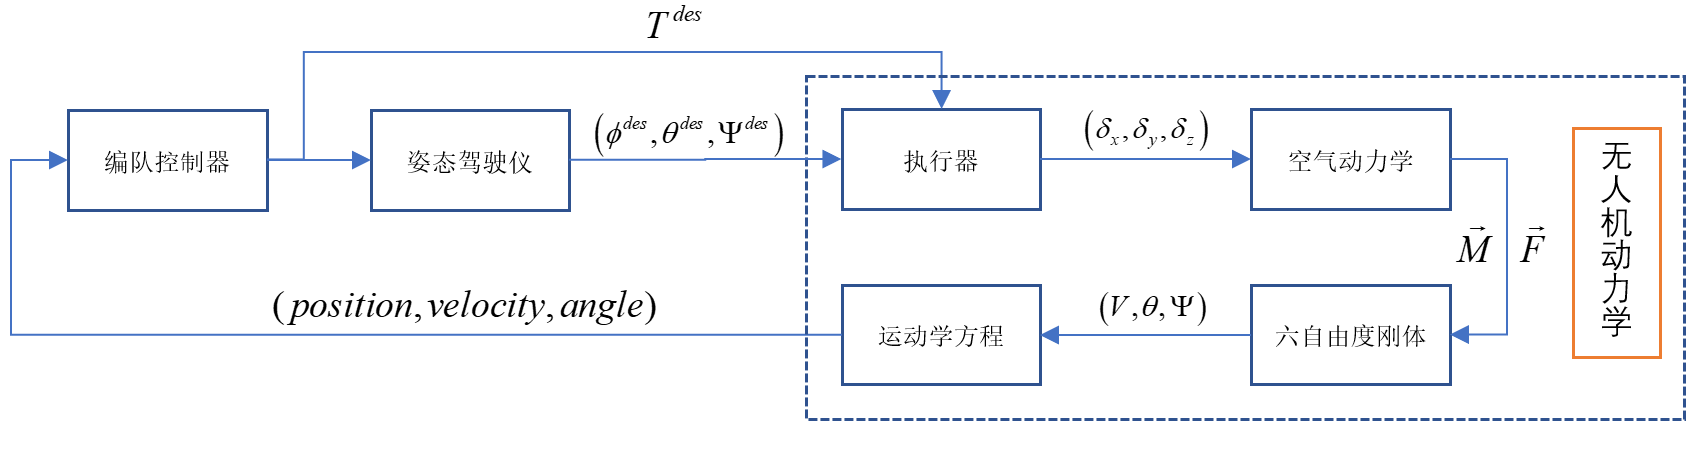
\includegraphics[width=0.85\textwidth]{figures/c3/c3-overview_controller.png}
    \caption{控制逻辑框图}\label{fig:c3-overview_controller}
\end{figure}
编队控制器的输入为定义的误差量,输出为无人机自动驾驶仪的内环输入值,即期望推力$T^{des}$,期望姿态$\Phi^{des},\theta^{des}$,偏航期望值$\Psi^{des}$将由内环姿态
自动驾驶仪按照协调转弯条件计算得到。本章的剩余部分将分别设计竖直平面以及水平平面的控制器。

需要说明的是:本章前两节先假设大气静止,设计无风条件下的编队控制器,第三节再引入风的干扰,并做相应处理。根据第二章的坐标系的定义,此假设将使得航迹坐标系与速度坐标系重合,又因为“无侧滑条件”(也称作协调转弯条件,BTT)的引入,机体二维水平平面坐标系$O_bx_by_b$将与前二者的水平平面坐标系($O_kx_ky_k$和$O_ax_ay_a$)重合。进而控制器产生的控制量与执行机构恰好对应,因此前两节之中,上述三种二维平面坐标系将不做区分。下面将选取航迹坐标系设计编队控制器。
\section{水平平面编队控制器设计}
\subsection{误差定义}
导航与制导的本质是控制地速的方向,实现手段是产生垂直于地速方向的法向加速度$a_{y_k}^{des}$;因而本章中误差以及控制量全部定义在航迹坐标系$O_kx_ky_kz_k$之中。但编队控制器不仅要控制速度的方向,还要控制速度的大小,以实现与领机的同步飞行。编队控制的最终目标为:
\begin{enumerate}
    \item 从机速度方向与领机的速度方向一致。
    \item 从机的速度大小与领机的速度大小一致。
    \item 从机的位置与从机的期望位置一致。
\end{enumerate}
此处产生三种误差类型,这三类误差均投影在从机航迹坐标系$O_kx_ky_kz_k$之中,便于之后对应要控制的物理量产生控制量:
\begin{enumerate}
    \item 领机与从机2维速度方向误差$\eta$,参见图\ref{fig:c02-2d_level_motion}。%TODO:记得改一下图,与之对应
    \item 领机与从机速度(地速$V_g$)大小误差$|V_g|^{err}$。
    \item 领机与期望位置3维误差$(P_{x_k}^{err},P_{y_k}^{err},P_{z_k}^{err})$
\end{enumerate}
因而此处水平平面的编队控制器的控制的任务是消除水平平面内的位置误差、速度大小以及速度方向误差,前两者在$O_kx_k$轴的分量需通过期望速度大小${|V|}_{x_k}^{des}$消除;前两者在$O_ky_k$轴
的分量,以及速度方向误差须通过期望法向加速度$a_{y_k}^{des}$消除。值得注意的是:实际上此处的速度方向误差代表了航迹系内的两分量之比值,实际上与角度误差代表同一误差,但是由于航迹系$O_kx_k$轴
的期望速度时刻变化,而所需的速度方向须按照领机速度方向一致,因而要控制速度的方向,而不是单纯的$O_kx_k$轴的速度分量。
\subsection{航迹系x轴方向控制器}
航迹系$O_kx_k$轴方向的控制器的输入为速度大小误差以及位置误差沿本轴分量的混合,控制器选用增量式离散$PID$控制器,最终的控制量的输出为航迹坐标系$O_kx_k$轴期望速度大小${|V|}_{x_k}^{des}$。控制器的表达式为:
\begin{equation}
    \left\{
    \begin{array}{l}
        |V_g|^{err}(k)=|V_g^{l}|(k)-|V_g^{f}|(k)\\
        P_{x_k}^{err}(k)=P_{x_g}^{des}(k)-P_{x_g}^{f}(k)\\
        e_{x_k}(k)=K_V|V_g|^{err}(k)+K_{Px}P_{x_k}^{err}(k)\\
        \begin{aligned}
        \Delta{|V|}_{x_k}^{des}(k)=&K_{p}^{xmix}[e_{x_k}(k)-e_{x_k}(k-1)]+K_{i}^{xmix}e_{x_k}(k)+\\
        &K_{d}^{xmix}[e_{x_k}(k)-2e_{x_k}(k-1)+e_{x_k}(k-2)]
        \end{aligned}
        \\
        {|V|}_{x_k}^{des}(k)=\Delta{|V|}_{x_k}^{des}(k)+{|V|}_{x_k}^{des}(k-1)
    \end{array}
    \right .
    \label{xk_vel_gen_equ}
\end{equation}
其中,前3式定义了混合误差形式,实际为速度误差与位置误差的线性叠加。后2式表示了最终的期望速度大小的产生。$k$为控制器第$k$次采样计算;$K_V,K_P$为误差线性混合常;$K_{p}^{xmix},K_{i}^{xmix},K_{d}^{xmix}$为增量式离散
$PID$控制器参数。

此处产生的期望速度大小,并不能直接为内环姿态驾驶仪所响应,需要经过竖直平面控制器的计算,位置误差$P_{z_k}^{err}$共同产生期望油门以及期望俯仰角。
\subsection{航迹系y轴方向控制器}
航迹系$O_ky_k$轴方向的控制器的输入为速度方向误差$\eta$以及位置误差的混合,类似于航迹系$O_kx_k$轴方向的控制器,控制器也选用增量式离散$PID$控制器,最终的输出为无人机滚转角期望值。
由图\ref{fig:c02-2d_level_motion}可得到:
\begin{equation}
    \eta^f=\Psi^l-\Psi^f
    \label{yaw_error}
\end{equation}
上式得到的是无人机速度方向的角度误差;

再考虑如图所示的无人机二维平面转弯运动:
\begin{figure}[H]
    \centering
    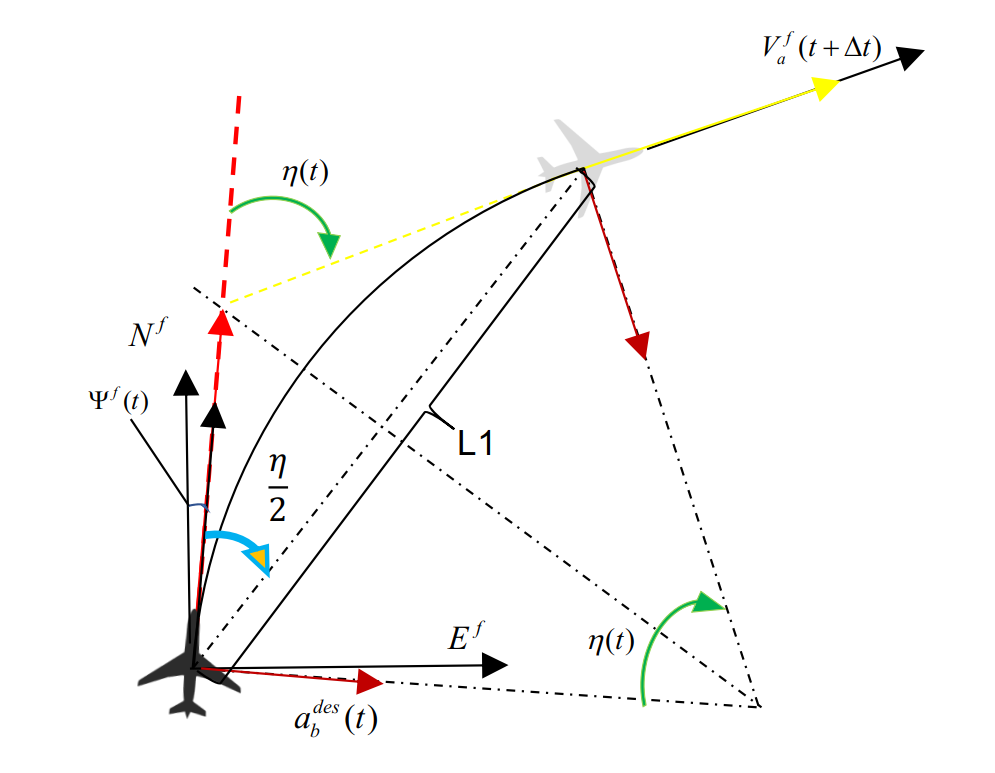
\includegraphics[width=0.5\textwidth]{figures/c3/c3-BTT.png}
    \caption{无人机二维平面转弯运动}\label{fig:c3-BTT}
\end{figure}
由于飞机速度的动力学惯性很大,在微分时间$\Delta t$时间内,速度的变化量可以忽略不计;在此时间内的偏航角增量为$\Delta\eta$,按照图中的几何关系,不难得到:
\begin{equation}
    a_{y_k}=V_g\dot{\eta}
    \label{btt_dot}
\end{equation}
上式即无人机期望偏航角速度与期望法向加速度关系。类似于上一节,定义混合误差为角度误差以及距离误差的线型混合。
再利用上一小节提出的增量式离散$PID$控制器,再综合式\ref{yaw_error},可得混合误差到期望法向加速度的表达式为:
\begin{equation}
    \left\{
        \begin{array}{l}
            \eta^f(k)=\Psi^l(k)-\Psi^f(k)\\
            P_{y_k}^{err}(k)=P_{y_g}^{des}(k)-P_{y_g}^{f}(k)\\
            e_{y_k}(k)=K_{\eta}\eta^f(k)+K_{Py}P_{y_k}^{err}(k)\\
                \begin{aligned}
                \Delta\dot{\Psi}^{des}(k)=&K_{p}^{ymix}[e_{y_k}(k)-e_{y_k}(k-1)]+K_{i}^{ymix}e_{y_k}(k)+\\
                &K_{d}^{ymix}[e_{y_k}(k)-2e_{y_k}(k-1)+e_{y_k}(k-2)]
                \end{aligned}\\
            \dot{\Psi}^{des}(k)=\Delta\dot{\Psi}^{des}(k)+\dot{\Psi}^{des}(k-1)\\
            \dot{\eta}^{des}(k)=-\dot{\Psi}^{des}(k)\\
            a_{y_k}^{des}(k)=-V_g^{f}(k)\dot{\eta}^{des}(k)
    \end{array}
\right .
    \label{angle_controller}
\end{equation}
上式得到的是期望法向加速度,再利用协调转弯(BTT)条件,将期望法向加速度,转化为期望滚转角:
\begin{equation}
    \tan\Phi^{des}(k)=\frac{a_{y_k}^{des}(k)}{g}
    \label{btt_a2roll}
\end{equation}
其中,$g$为当地重力加速度常量。至此,水平平面面内可计算得到无人机的期望滚转角$\Phi^{des}$以及期望速度大小$|V|_{x_k}^{des}$
\section{竖直平面编队控制器设计}
竖直平面编队控制器的输入为期望速度大小$|V|_{x_k}^{des}$以及期望高度(实际代表了高度误差$P_{z_b}^{err}$),输出为期望俯仰角$\theta^{des}$以及期望推力$T^{des}$。控制器选用基于能量的总能量控制法
(total energy control system,$TECS$)。固定翼无人机的速度控制和高度控制是耦合的,即单独控制高度或速度时,另一个未被控制量将会发生变化:
下面通过飞机飞行动力学纵向运动方程简单说明:
\\方程组\ref{fol_motion_eauation1}的第三式说明:飞机高度方向的变化率与地速大以及俯仰角大小有关,且为正相关。
\\根据飞机飞行动力学,无人机纵向运动质心运动的动力学方程为:
\begin{equation}
    \left\{
    \begin{aligned}
    &m \frac{\mathrm{d} V}{\mathrm{d} t}=T \cos (\alpha+\varphi) \cos \beta-D-m g \sin \gamma\\
    &m V \cos \gamma \frac{\mathrm{d} \chi}{\mathrm{d} t}=T[\sin (\alpha+\varphi) \sin \mu-\cos (\alpha+\varphi) \sin \beta \cos \mu]+C \cos \mu+L \sin \mu\\
    &-m V \frac{\mathrm{d} \gamma}{\mathrm{d} t}=T[-\sin (\alpha+\varphi) \cos \mu-\cos (\alpha+\varphi) \sin \beta \sin \mu]+\operatorname{Csin} \mu-L \cos \mu+m g \cos \gamma
    \end{aligned}
    \right .
    \label{point_dynamaic}
\end{equation}
其中,$\alpha,\mu,\phi$分别为迎角,速度滚转角以及发动机安装角。
根据之前的假设,可以将第一式近似作:
\begin{equation}
    m \frac{\mathrm{d} V}{\mathrm{d} t}=T-D-m g \sin \theta
    \label{1st_point_dynamaic}
\end{equation}
综合\ref{1st_point_dynamaic}、\ref{fol_motion_eauation1}两式,可以得到如下关于速度以及高度通道的控制逻辑图:
\begin{figure}[H]
    \centering
    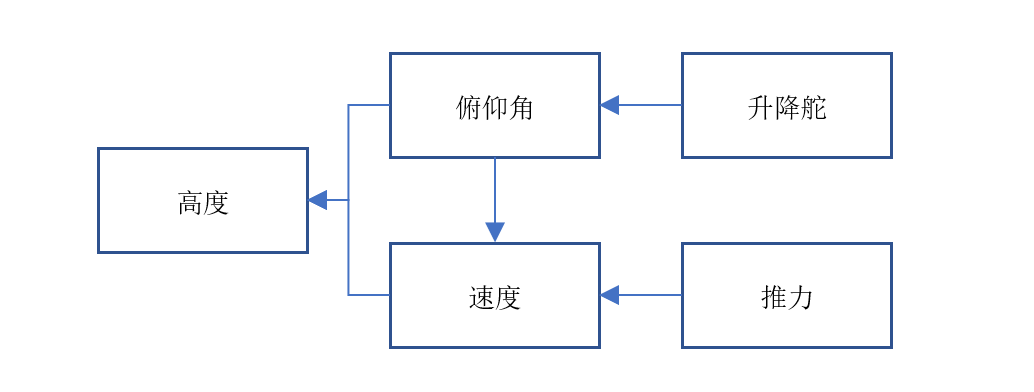
\includegraphics[width=0.75\textwidth]{figures/c3/relation_theta_thrust}
    \caption{速度以及高度通道的控制逻辑图}\label{fig:relation_theta_thrust}
\end{figure}
因而速度和高度需要同时考虑,相应的,期望俯仰角以及推力也需要同时计算。$TECS$控制器正是为此种情况设计的:%TODO:需要添加引用
所谓总能量控制(total energy control)是将无人机的速度以及高度计算得到相应的动能以及势能作为直接控制对象,应用PID控制器对动能与势能的和(total energy)
以及动能与势能的转化(total energy balance)进行控制,计算得到无人机期望俯仰角以及期望推力的控制器。飞机作为一个动力学系统,其机械能来自推力做功的输入,因而总能量控制对应着期望推力;与之对应的俯仰角控制是能量守恒的,
可作为动能向势能(反之亦然)的转化途径,对此种能量转化的控制对应着期望俯仰角。下面简要介绍$TECS$控制器的计算过程:
\\
无人机的总能量为:
\begin{equation}
    E_T=\frac{1}{2}mV_T^2+mgh
    \label{ET}
\end{equation}
对上式两边微分,可得到总能量变化率:
\begin{equation}
    \dot{E_T}=mV_T\dot{V_T}+mg\dot{h}
    \label{ET_rate}
\end{equation}
由此可得单位总能量变化率:
\begin{equation}
    \dot{E}=\frac{\dot{E}_{T}}{m g V_{T}}=\frac{\dot{V}_{T}}{g}+\frac{\dot{h}}{V_{T}}=\frac{\dot{V}_{T}}{g}+\sin \gamma
    \label{specif_ET_rate}
\end{equation}
更换式\ref{point_dynamaic}第一式形式,可得到:
\begin{equation}
    T-D=m g\left(\frac{\dot{V}_{T}}{g}+\sin \gamma\right)
    \label{point_dynamaic_change}
\end{equation}
由此可得:
\begin{equation}
    \Delta T=m g\left(\frac{\dot{V}_{T}}{g}+sin\gamma\right)
    \label{thrust}
\end{equation}
关于能量转化,定义:
\begin{equation}
    B=m g h-\frac{1}{2} m V_{T}^{2}
\end{equation}
能量转化率为:
\begin{equation}
\dot{B}=sin\gamma-\frac{\dot{V}_{T}}{g}
\end{equation}
这里参照开源软件$PX4$内部的TECS控制器设计方法,总能量环和能量分配环的控制逻辑框图如下所示:
\begin{figure}[H]
    \centering
    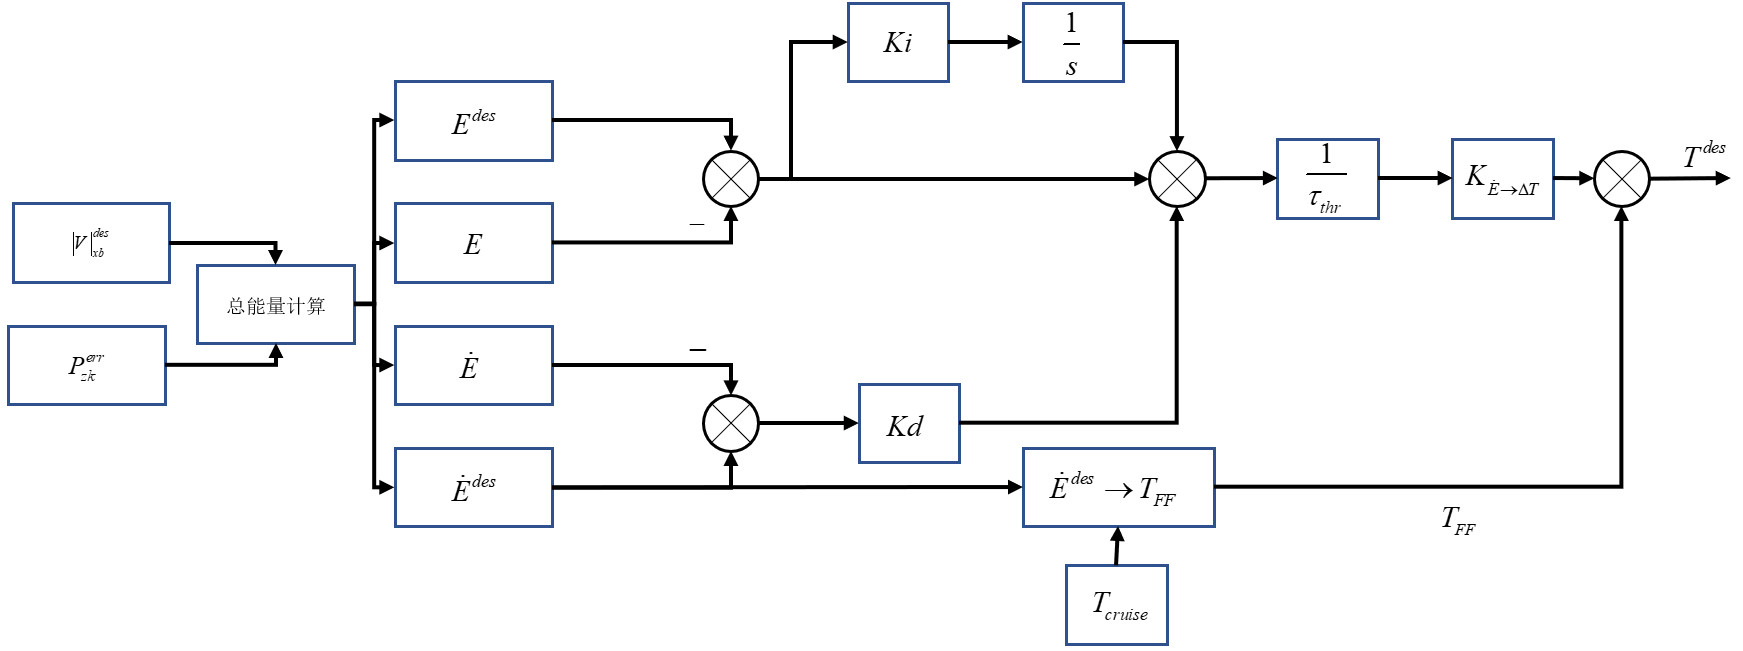
\includegraphics[width=0.9\textwidth]{figures/c3/TECS_throttle.jpg}
    \caption{总能量环}\label{fig:total_energy}
\end{figure}
\begin{figure}[H]
    \centering
    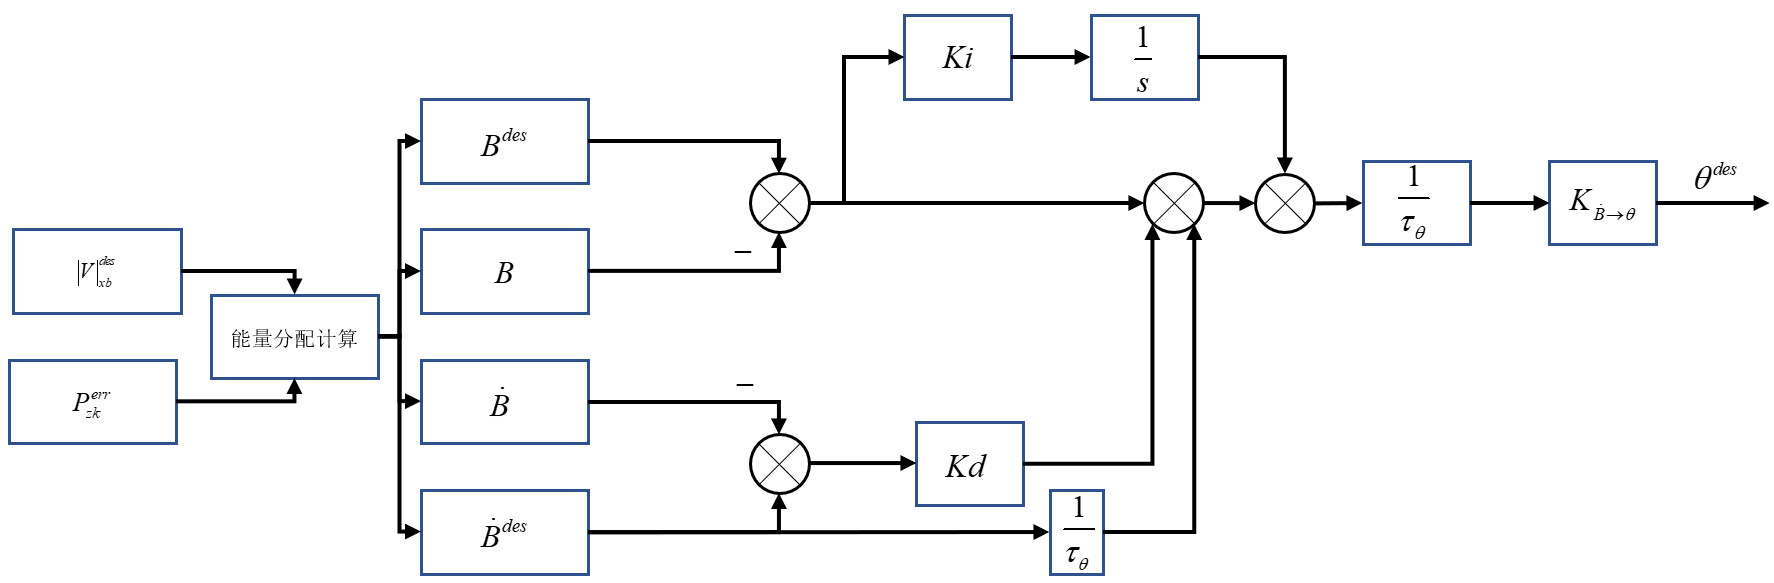
\includegraphics[width=0.9\textwidth]{figures/c3/TECS_pitch.jpg}
    \caption{能量分配环}\label{fig:balance_energy}
\end{figure}
图\ref{fig:total_energy}中,$K_i,K_d,T_{FF},\tau_{thr},K_{\dot{E}\rightarrow\Delta T}$分别为积分项,微分项比例系数,油门前馈项,油门时间常数以及比例向项系数。
图\ref{fig:balance_energy}中,$K_i,K_d,\tau_{\theta},K_{\dot{B}\rightarrow\Delta \theta}$分别为积分项,微分项比例系数,俯仰角时间常数以及比例向项系数。

至此,来自水平平面的期望速度$|V|_{x_k}^{des}$以及纵向平面的位置误差$P_{z_k}^{err}$将转化为期望俯仰角以及期望推力进入内环姿态驾驶仪;水平平面编队控制器
产生的期望滚转角也将进入姿态驾驶仪内环。内环姿态自动驾驶仪首先按照无侧滑条件得出期望偏航角速度$\dot{\Phi}^{des}$,然后再利用串级PID分角速度环,角
加速度环计算得到期望的执行机构的偏转角度。但现在的编队控制器还不足以直接用来进行编队控制实现,还需要经过一定的工程处理,详见下一节。
\section{实际应用时的考虑}
在实际应用编队控制器时,按照已有的经验,应主要考虑以下几个方面:
\begin{enumerate}
    \item 在无人机距离期望位置较远以及相对较近时,控制的目的是不完全一致的;应根据不同的控制需求分段设计控制律。
    \item 无人机的空速与地速差距较大(风速很大)时,地速与空速方向不能简单认为一致,应分析之后做相应的处理。
    \item 考虑到无人机各个动力学量的范围,应按照前期对于飞行平台飞行性能计算的结果对控制器计算过程中的各个物理量进行实际限幅。
    \item 无人机原始信息两量测噪声问题,应设计便于使用的滤波器加以滤波。
\end{enumerate}
下面按照上述问题介绍相应的解决方法:

\subsection{编队控制器分段设计} 
在位置误差较大时,编队控制器的主要目的应为:以最大速度飞行,迅速减小距离误差;此时无人机速度的期望方向应时刻指向期望点而并非领机的速度方向。选择水平距离误差大小作为分段控制器的分段依据,定义水平距离误差为$|P|_{2d}^{err}(k)=\sqrt{[P_{x_k}^{err}(k)]^2+[P_{y_k}^{err}(k)]^2}$,决断距离记作$|P_0|_{2d}^{err}$。于是可以得到以下期望速度的表达式:
\begin{equation}
    |V|_{x_k}^{des}(k)=
    \begin{cases}
        V_{max}^f& |P|_{2d}^{err}(k)>|P_0|_{2d}^{err}\\
        \Delta{|V|}_{x_k}^{des}(k)+{|V|}_{x_k}^{des}(k-1)& |P|_{2d}^{err}(k)\leq|P_0|_{2d}^{err}
    \end{cases}
    \end{equation}
第二阶段的期望速度速度产生详见式\ref{xk_vel_gen_equ}。
关于此阶段的法向加速度的产生,此处使用××等人提出的L1控制器,将L1距离选为从机当前位置与期望位置的距离误差。其表达式如下:
\begin{equation}
    a_{y_k}^{des}(k)=
    \begin{cases}
        2\frac{V^2}{L_1}\sin{\frac{\eta}{2}}& |P|_{2d}^{err}(k)>|P_0|_{2d}^{err}\\
        -V_g^{f}(k)\dot{\eta}^{des}(k)& |P|_{2d}^{err}(k)\leq|P_0|_{2d}^{err}
    \end{cases}
    \end{equation}
上式中各运动学量参见图\ref{fig:c3-BTT},第二阶段法向加速度的产生详见式\ref{angle_controller}。再配合固定翼无人机协调转弯条件(式\ref{btt_a2roll}),可得到分段之后的期望滚转角。
\subsection{风速较大时的处理} 
\subsubsection*{风速因素对于编队控制器的影响分析}
无论导航与制导还是编队的期望速度均是对无人机的地速而言的。当内环姿态驾驶仪以无侧滑条件为基础时,若控制效果较好,则可保证侧滑角$\beta\approx 0$,即:无人机在水平二维平面运动时,空速方向与机身纵轴在同一竖直平面内。因而飞机在平飞时,空速方向几乎与机身纵轴重合。无论有风还是无风,均有上述结论。

参照图\ref{fig:c02-2d_level_motion},当风速$V_{wind}^f$较小时,空速与地速几乎重合,且等大,此时直接将空速方向认为与空速方向一致,进而与机体方向一致的做法是可行的:前文提出的位置、角度以及速度误差均投影在航迹系$O_kx_ky_kz_b$中,所产生的修正信号$|V|_{x_k}^{des}(k),a_{y_k}^{des}(k)$与体轴系的$O_bx_b$以及$O_by_b$几乎重合,i控制机构(油门,副翼)直接相应控制信号即可,符合前文的设计。

但当风速较大时(例如,风速大小已经超过了地速的$\frac{1}{3}$,且与飞机地速有一定的角度),则会出现如下图所示的情况:
\begin{figure}[H]
    \centering
    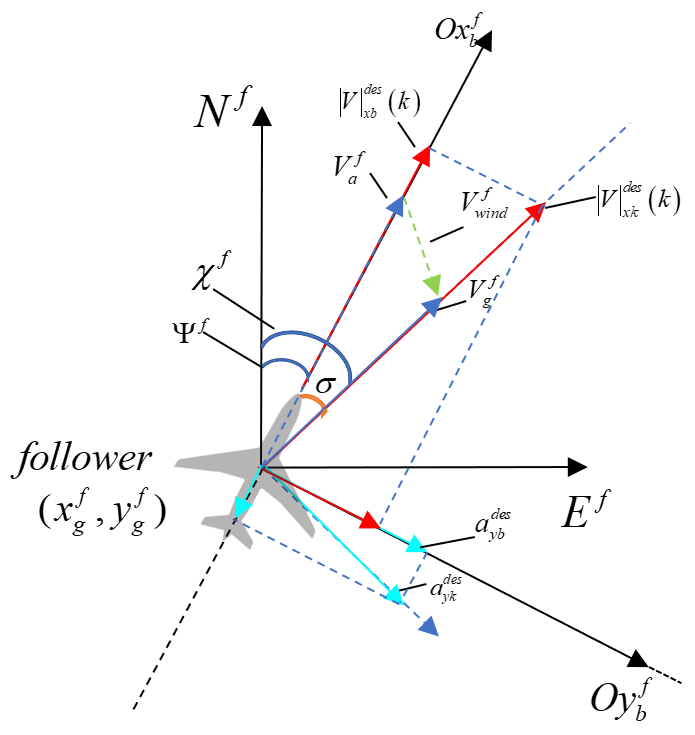
\includegraphics[width=0.5\textwidth]{figures/c3/heavy_wind.png}
    \caption{空速与地速之差较大}\label{fig:heavy_wind}
\end{figure}
图中,风速的大小以及方向已经不能忽略不计,可以得出。原始产生在航迹坐标系$O_kx_ky_kz_k$中的期望速度以及期望与执行机构(油门以及副翼)所在的机体系已有大小为$\sigma$的夹角。
\subsubsection*{风速较大时的改进}
如图\ref{fig:heavy_wind}所示,原始在航迹坐标系之中产生的控制量的期望值若要在机体系之中产生正确的相应,需要进行相应的坐标变换。
\begin{equation}
    \left[
    \begin{matrix}
        control\_input\_x_b(k)\\
        control\_input\_x_y(k)
    \end{matrix}
    \right]
    =  
    \left[  
    \begin{matrix}
        cos\sigma& -sin\sigma\\
        sin\sigma& cos\sigma
    \end{matrix}
    \right]
    \left[
        \begin{matrix}
            |V|_{x_k}^{des}(k)\\
            a_{y_k}^{des}(k)
        \end{matrix}
        \right]
\end{equation}
但是由于机体系两个通道所能够接受的的控制量并不是一致的,需要进行工程化处理:
\begin{equation}
    \left\{
        \begin{aligned}
            &control\_input\_x_b(k)=cos\sigma|V|_{x_k}^{des}(k)+\sum_{n=1}^k\{-sin[\sigma(n)]a_{y_k}^{des}(n)T\}\\
            &control\_input\_x_y(k)=\frac{1}{T}\{sin[\sigma(k)|V|_{x_k}^{des}(k)]-sin[\sigma(k-1)|V|_{x_k}^{des}(k-1)]\}+cos\sigma a_{y_k}^{des}(k)
        \end{aligned}
    \right .
\end{equation}
上式中,$T$是控制时间间隔。实际应用时上式中的微分项要考虑低通滤波以及时间间隔问题,积分项应考虑积分饱和问题。
\subsection{无人机飞行性能限幅设计}
考虑到实际系统各个环节的有界性问题,需要按照无人机气动外形尺寸以及基本飞机空气动力学,计算得出的无人机飞行性能参数,作为实际控制时的各个环节物理量的限幅依据。表\ref{tab:takeoff_performance}-\ref{tab:sink_performance}展示了飞机部分飞行性能:
\begin{table}[H]
    \centering
    \caption{无人机起飞、爬升性能} \label{tab:takeoff_performance}
    \begin{tabular*}{0.9\textwidth}{@{\extracolsep{\fill}}c|ccccccc}
    \toprule
        飞行性能&抬轮速度&起飞速度&滑跑距离&起飞时间
        &爬升率&爬升角
        \\
    \midrule
        值&$4.82m/s$&$5.52m/s$&$16.45m$&$7.36s$
        &$5.99m/s$&$31.21°$\\
    \bottomrule
\end{tabular*}
\end{table}
\begin{table}[H]
    \centering
    \caption{无人机平飞性能} \label{tab:task_performance}
    \begin{tabular*}{0.9\textwidth}{@{\extracolsep{\fill}}c|cccc}
    \toprule
        飞行性能&平定常飞空速&最大空速&最小空速&失速迎角%TODO:需要有最大前项加速度
        \\
    \midrule
        值&$11.52m/s$&$43.76m/s$&$4.60m/s$&$9.94°$\\
    \bottomrule
\end{tabular*}
\end{table}
\begin{table}[H]
    \centering
    \caption{无人机机动性能} \label{tab:motive_performance}
    \begin{tabular*}{0.9\textwidth}{@{\extracolsep{\fill}}c|ccccc}
    \toprule
        飞行性能&转弯速率&转弯半径&转弯时间&法向过载系数&最大滚转角%TODO:需要有最大滚转角速度
        \\
    \midrule
        值&$11.56m/s$&$14.31m/s$&$7.80s$&$1.38$&$43.56°$\\
    \bottomrule
\end{tabular*}
\end{table}
\begin{table}[H]
    \centering
    \caption{无人机下降、爬降落性能} \label{tab:sink_performance}
    \begin{tabular*}{0.9\textwidth}{@{\extracolsep{\fill}}c|cccc}
    \toprule
        飞行性能&下降率&下降角&降落速度&滑跑距离
        \\
    \midrule
        值&$10.19m/s$&$60.15m/s$&$5.89m/s$&$14.81m$
        \\
    \bottomrule
\end{tabular*}
\end{table}
\subsection{原始数据滤波器设计}
此处所涉及的原始数据,主要是来自领机以及从机的空速计测量的空速信息。此处使用一阶低通滤波器来实现对于空速信息的滤波。下面简单介绍一阶低通滤波器:
一阶低通滤波器又称作一阶惯性滤波器,传递函数形式为标准一阶惯性环节:
\begin{equation}
    V_0=\frac{1}{1+\tau j\omega}
\end{equation}
其中$\tau$是时间常数。转换成时域形式:
\begin{equation}
    V_0=V_i -\tau\frac{dV_0}{dt}
\end{equation}
离散化之后:
\begin{equation}
    V_0(k)=\frac{V_i(k)+\frac{\tau}{T}V_0(k-1)}{1+\frac{\tau}{T}}
\end{equation}
其中,$T$为控制器时间间隔,$T=\frac{1}{f}$。
此种滤波器在使用时需要注意时间常数的选择,时间常数过大,虽然数据波形会相对平滑,但是滞后较为严重。

\chapter{无人机编队整体控制逻辑、仿真环境以及硬件选型}
\label{chap:hardware}
本章主要介绍无人机编队的编队控制算法之外的系统组成部分;之后介绍无人机编队的整体的控制的实现逻辑,之后将介绍无人机编队的动力学仿真环境的搭建。
最后将介绍本次设计之中所用到的无人机型号,自动驾驶仪硬件以及姿态自动驾驶仪内环基本控制逻辑。
\section{无人机编队软件整体控制逻辑}
本部分将介绍完整的软件的控制逻辑以及使用的软件环境。
内环姿态驾驶仪使用的是开源自动驾驶仪PX4。PX4是一个为无人机或者其他无人系统设计的高度模块化、可定制化的开源自动驾驶仪软件系统;
PX4软件本身提供了丰富的应用程序接口(API)以及软件开发工具包(SDK),可以与$ROS$等机器人操作系统进行数据交互。下图展示了$PX4$
的软件架构:
\begin{figure}[H]
    \centering
    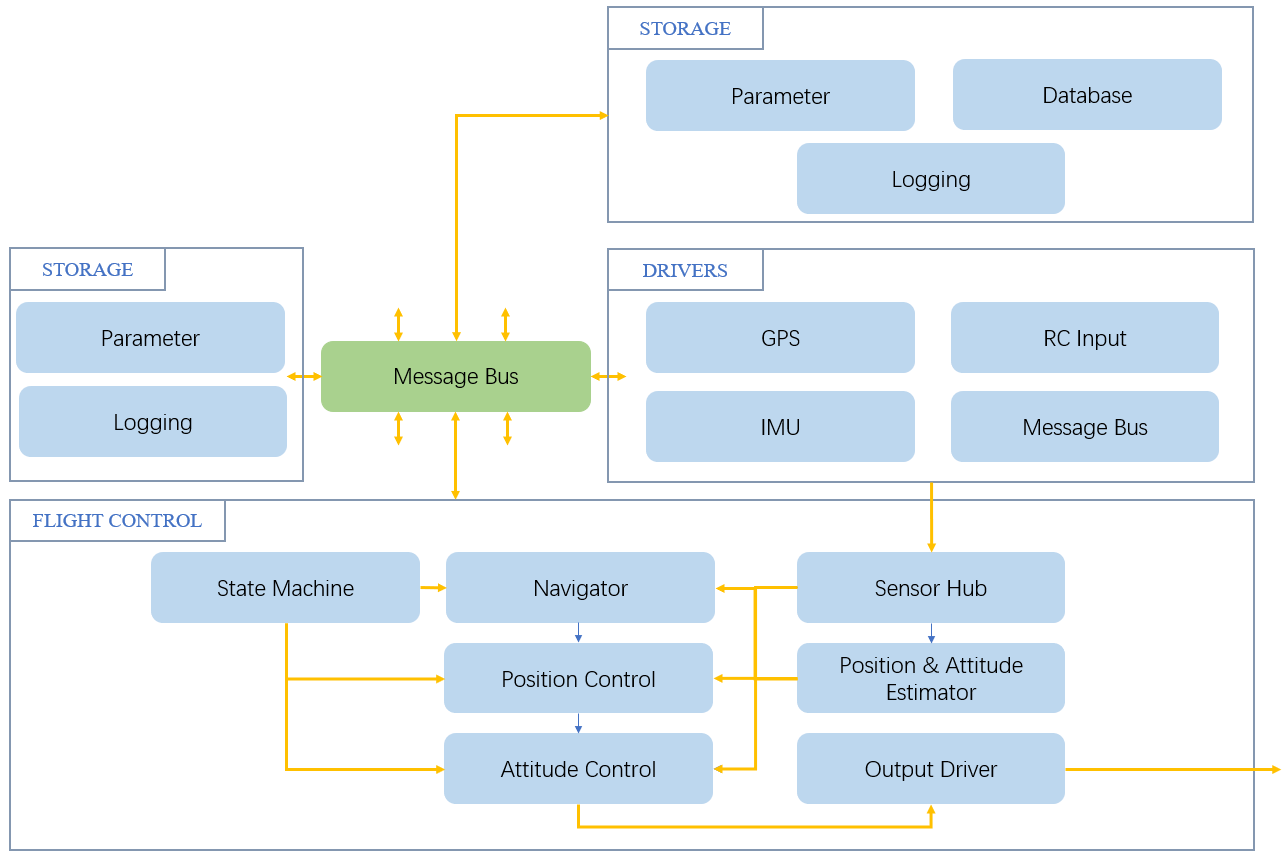
\includegraphics[width=0.8\textwidth]{figures/c4/PX4_archticher.png}
    \caption{PX4软件架构}\label{fig:PX4_archticher.png}
\end{figure}

编队控制算法所运行的软件环境是$ROS$($Robot$ $Operating$ $System$)。$ROS$是一个适用于机器人的开源操作系统。
它提供了操作系统应有的服务,包括硬件抽象,底层设备控制,常用函数实现,进程间消息传递,以及包管理。
它也提供用于获取、编译、编写、和跨计算机运行代码所需的工具和库函数。本次使用的应用程序接口是$ROS$下的$mavros$功能包,
本功能包的作用是:将来自自动驾驶仪的无人机状态数据由$mavlink$通信协议转换为$ROS$的进程间的通讯的协议;
将来自编队控制器的姿态驾驶仪内环的期望姿态角以及期望油门值按照$mavlink$的协议进行编码,从而起到沟通编队控制器以及姿态驾驶仪内环的桥梁作用。
\section{无人机软硬件环境选配}
本文所设计的编队控制器是以开源自动驾驶仪$PX4$的内环为基础的,$PX4$的内环自动驾驶仪运行在$Pixhawk$这一开源硬件之上,成为上层控制的下位机(slave computer):
编队控制算法运行在具有$ROS$环境的上位机(host computer)中;
整体的软件硬件选配关系如下图所示:
\begin{figure}[H]
    \centering
    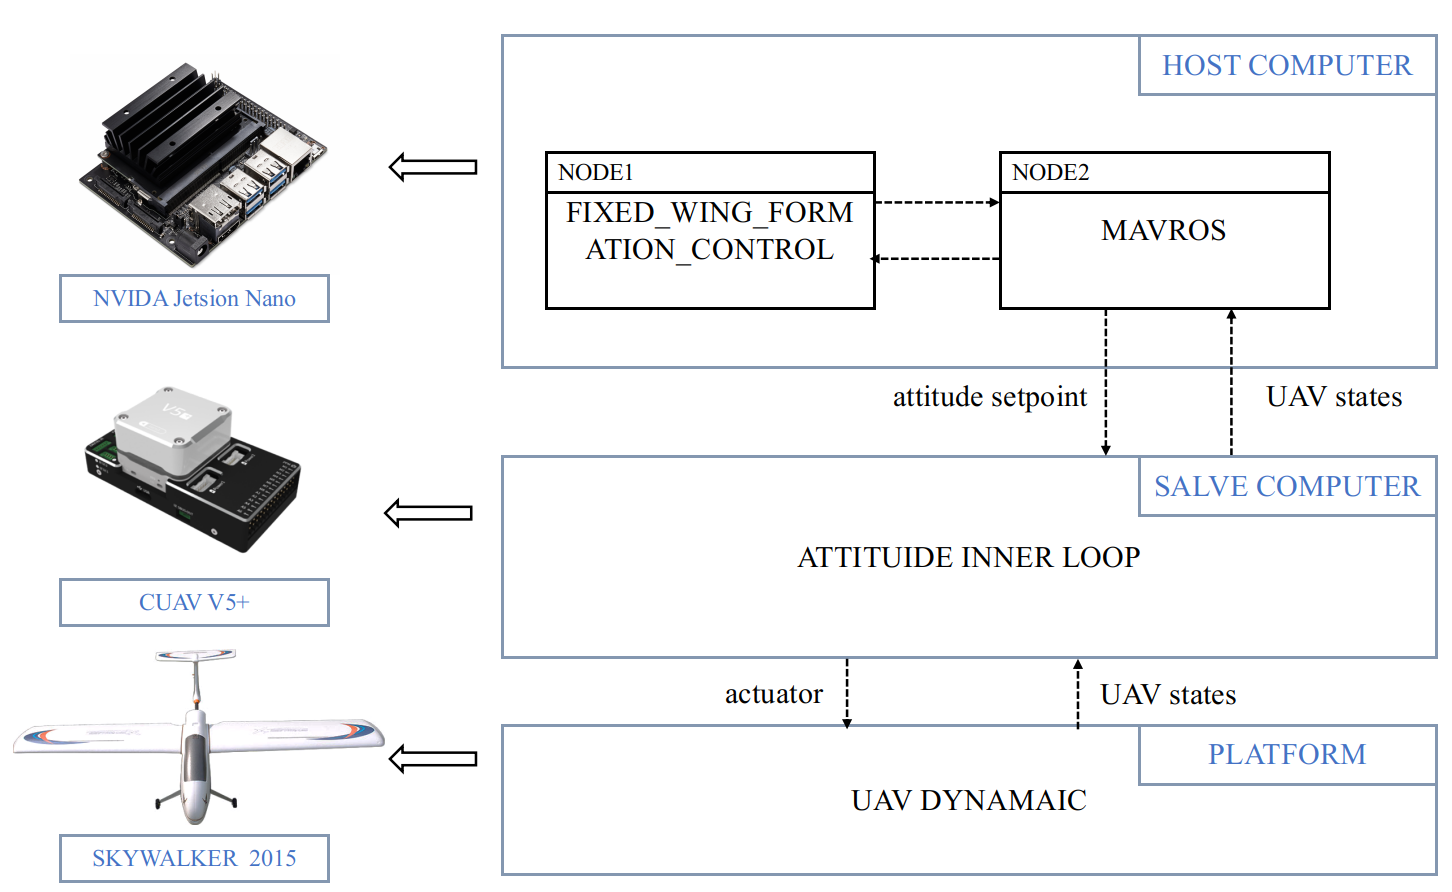
\includegraphics[width=1\textwidth]{figures/c4/c4-soft-hard.png}
    \caption{硬件软件选配关系}\label{fig:c4-soft-hard.png}
\end{figure}
\section{无人机编队动力学仿真环境}
所谓无人机动力学仿真环境,是在考虑无人机的空气动力的作用基础基础之上搭建的仿真环境,相较于控制器的数学仿真,此种仿真环境考
虑了无人机作为一个实际的被控系统而存在的过渡过程,不确定性以及扰动因素,将更加符合无人机飞行时的实际状态。
本次动力学仿真环境基于$Gazebo$这一通用的开源仿真环境仿真环境的。
\begin{figure}[H]
    \centering
    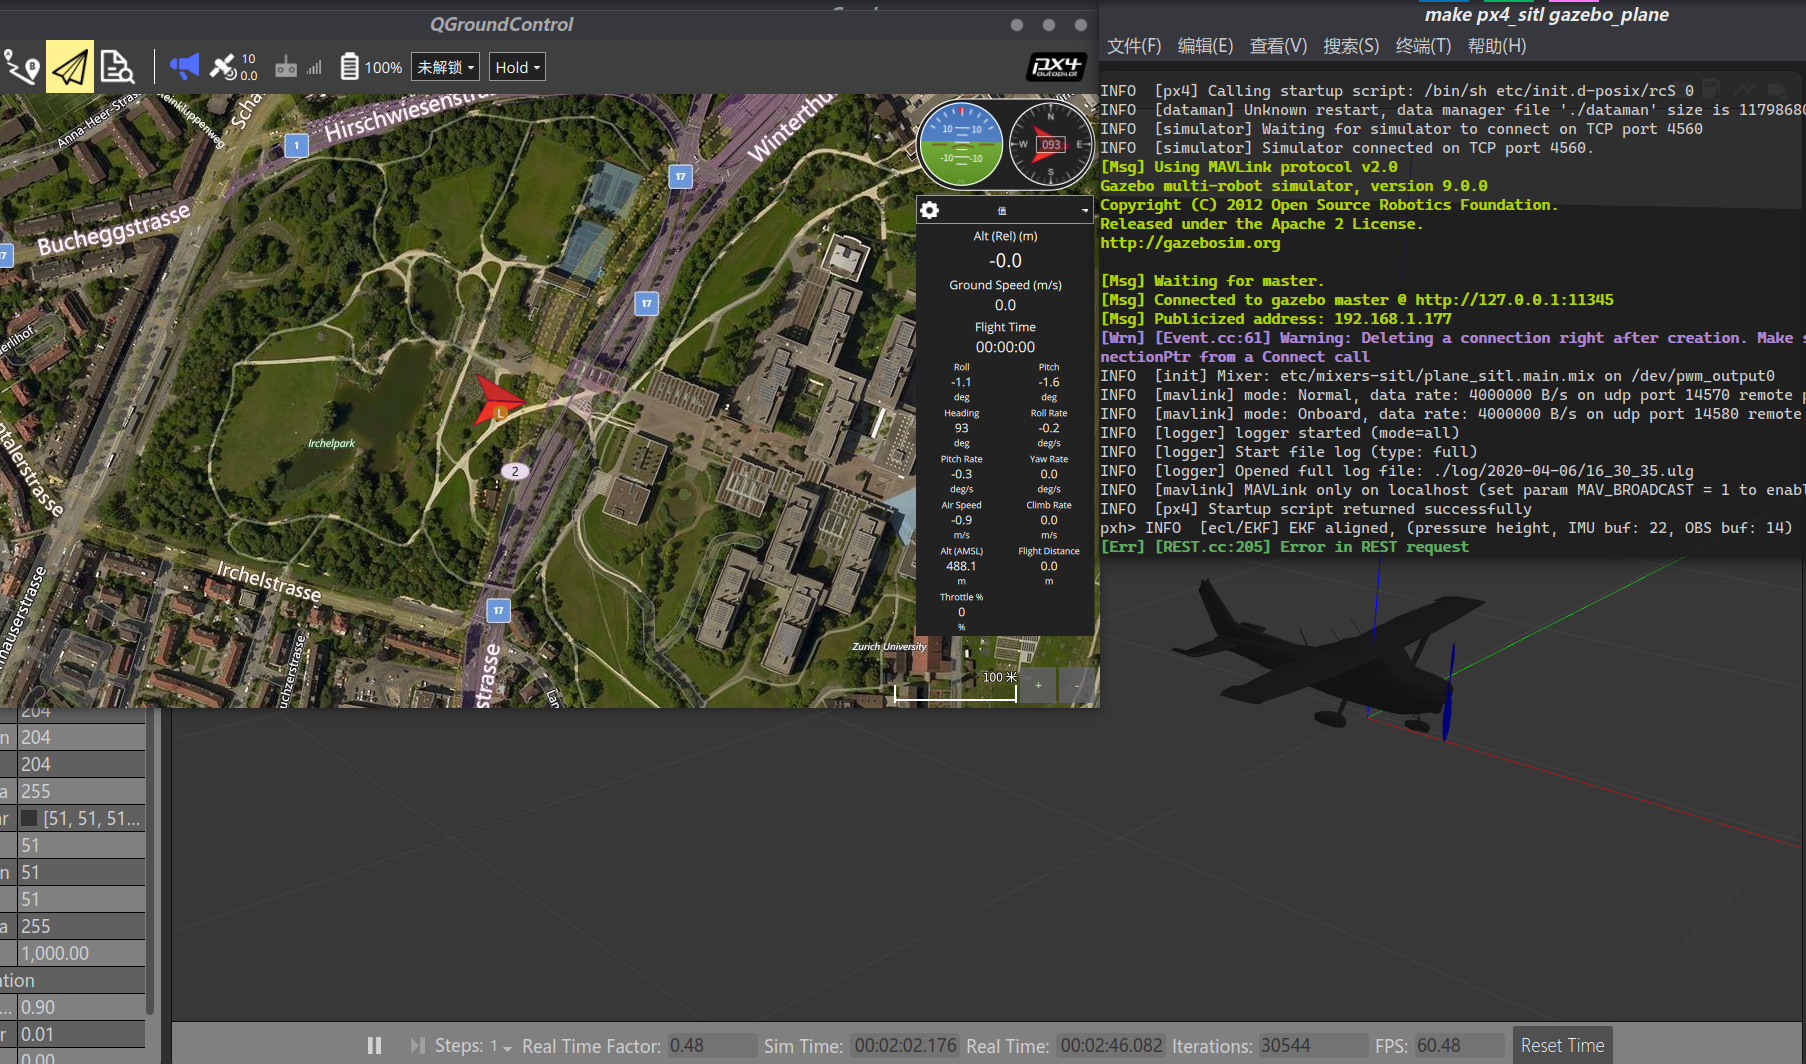
\includegraphics[width=0.75\textwidth]{figures/c4/Gazebo.png}
    \caption{Gazebo仿真环境}\label{fig:c4-Gazebo}
\end{figure}

仿真之中的飞机的动力学模型由Gazebo仿真环境给出,可自定义飞机的质量,推力等参数;仿真之中的传感器数据由Gazebo产生,由PX4读取,作为
真实环境之中的传感器数据的仿真。基于$ROS$的编队控制程序同时运行,通过mavros等程序API进行数据交互,完成动力学仿真。
相应的仿真程序之间的逻辑关系如下图所示:
\begin{figure}[H]
    \centering
    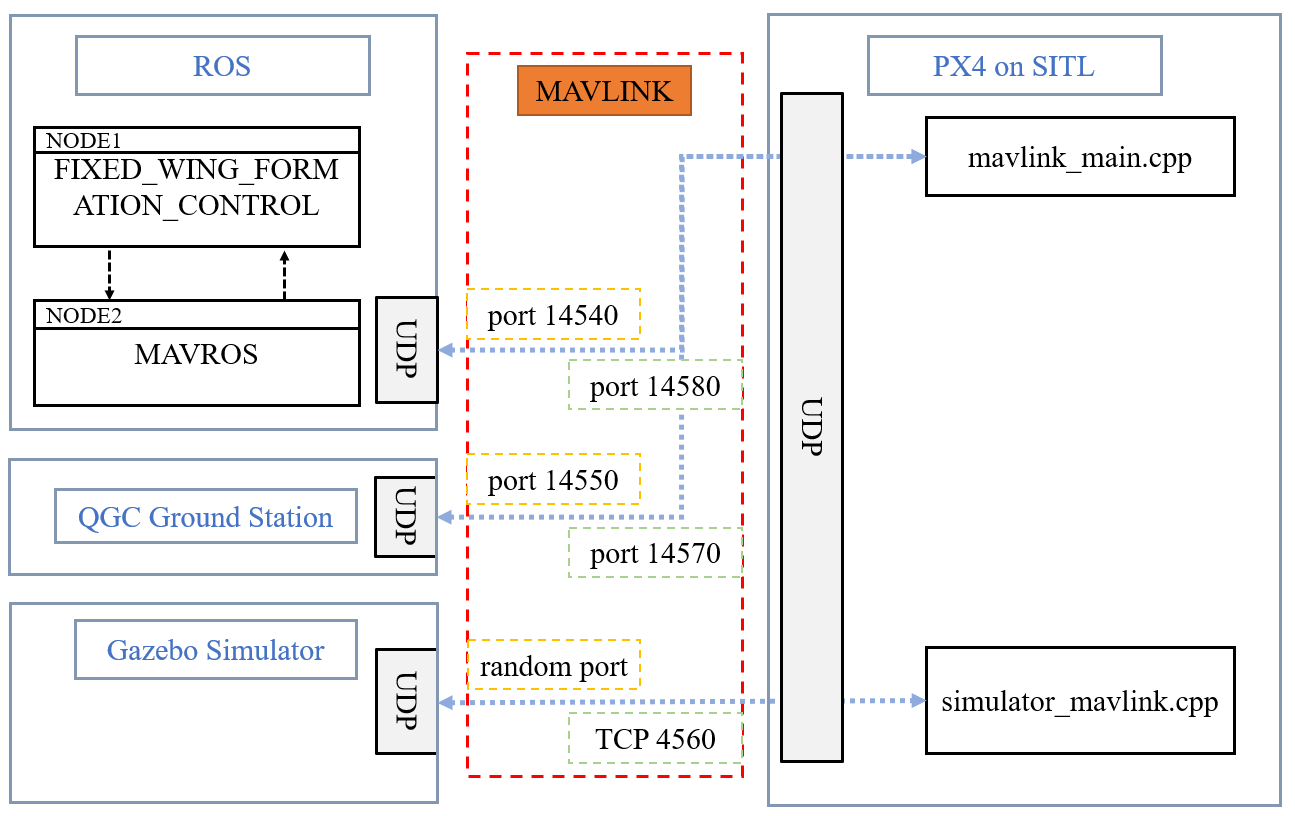
\includegraphics[width=0.75\textwidth]{figures/c4/px4_sitl_overview.png}
    \caption{编队控制仿真逻辑}\label{fig:px4_sitl_overview}
\end{figure}

\chapter{控制器仿真以及实际飞行实验结果分析}
\label{chap:simulatin_expermient}
本章之中,按照第\ref{chap:controller_design}
章中给出的控制器的数学模型,选定相应的初始条件进行双机的质点模型数学仿真:即不考虑无人机的姿态,只考虑无人机的位置,速度大小以及方向。之后,利用第\ref{chap:hardware}章中介绍的$ROS/Gazebo-PX4$仿真环境,在考虑无人机动力学的条件下进行双机编队仿真。
\section{基于MATLAB/Simulink的双机编队数学仿真}
本节数学仿真只验证编队控制器的控制性能以及控制逻辑的正确性,因而在仿真之前,做如下假设:
\begin{enumerate}
\item 无人机自动驾驶仪内环仅为一个具有时间常数$\tau$一阶惯性环节。
\item 无人机的姿态动力学没有过渡过程,即姿态动力学方程由相应的稳态方程代替。
\end{enumerate}
另外,按照第\ref{chap:controller_design}章中控制器设计分为水平平面以及竖直平面的原则,本节之中的仿真也是分为两个方面进行的;在任何
在其中任意一个平面内仿真时,都假设另外一个平面已经达到了控制目标,并且处于稳态。

在水平面的仿真中:选取的初始条件均为在地面坐标系$NED$中定义:
领机初始位置$P_{0}^{l}=(0,100)$;
领机初始速度$V_{0}^{l}=(20,0)$;
从机的初始位置$P_{0}^{f}=(0,0)$;
从机的初始速度$V_{0}^{f}=(10,10)$;
仿真的结果如下三图所示:其中,图\ref{fig:c5-matlab-pos},表示双机编队位置关系,横轴为NED坐标系下的E轴,纵轴为N轴。
图\ref{fig:c5-matlab-vel}以及图\ref{fig:c5-matlab-eta}分别表示双机速度大小以及速度方向的与时间的关系图。由仿真结果可得,
在算法层面上,第\ref{chap:controller_design}所设计的编队控制器在水平平面内可以完成编队控制的任务。
\begin{figure}[H]
    \centering
    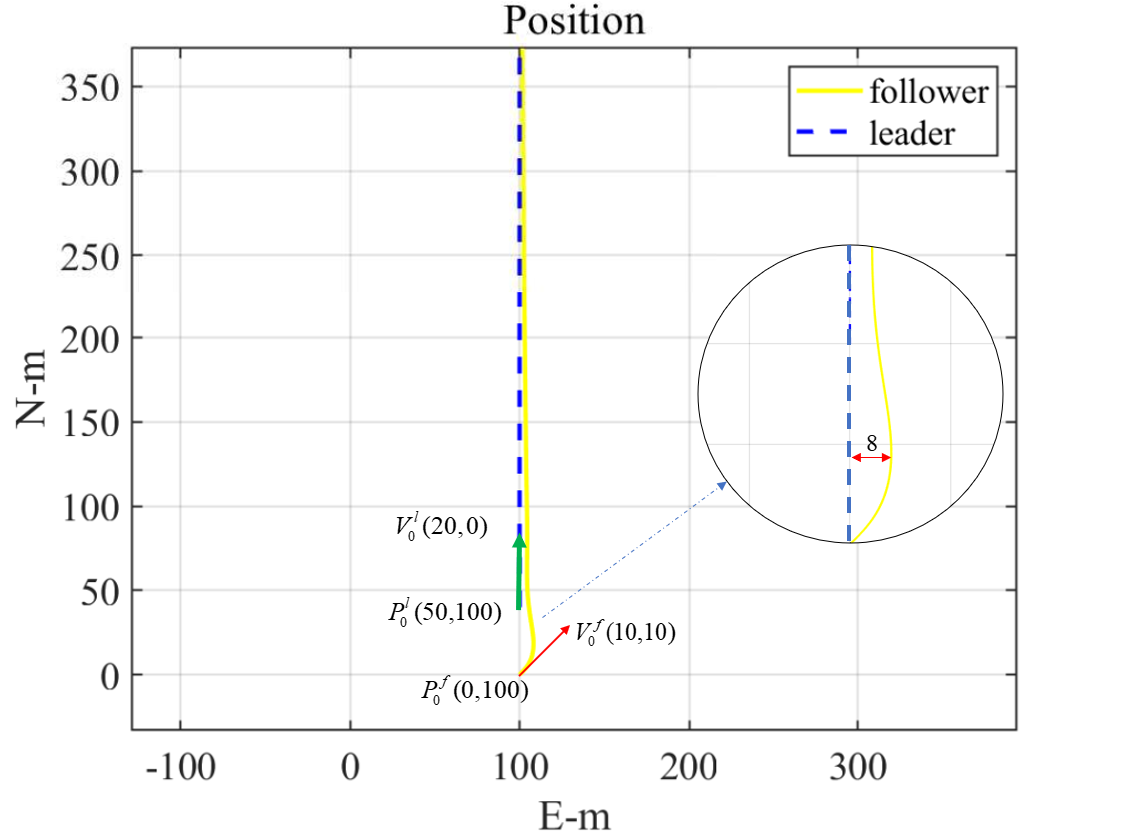
\includegraphics[width=0.85\textwidth]{figures/c5/c5-matlab-pos.png}
    \caption{水平面双机编队位置关系}\label{fig:c5-matlab-pos}
\end{figure}
\begin{figure}[H]
    \centering
    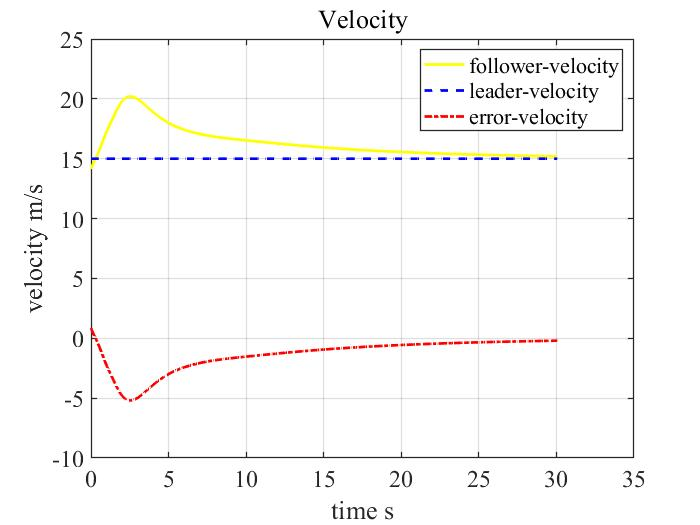
\includegraphics[width=0.85\textwidth]{figures/c5/c5-matlab-vel.jpg}
    \caption{水平面双机速度关系}\label{fig:c5-matlab-vel}
\end{figure}
\begin{figure}[H]
    \centering
    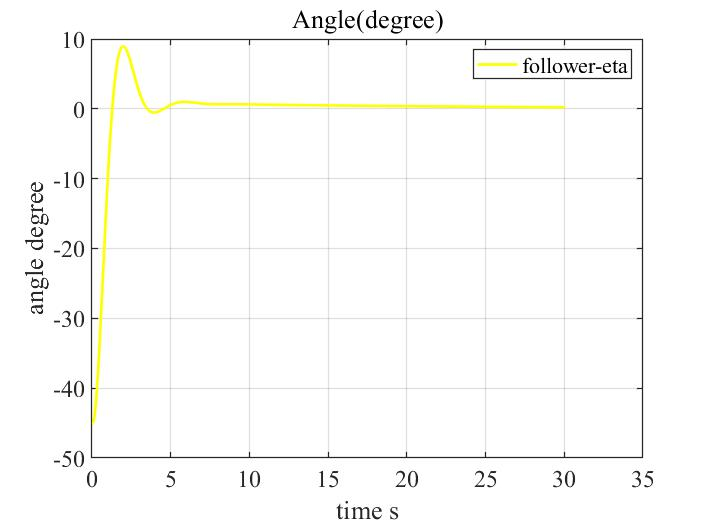
\includegraphics[width=0.85\textwidth]{figures/c5/c5-matlab-eta}
    \caption{水平面双机速度方向关系}\label{fig:c5-matlab-eta}
\end{figure}

竖直平面内,由于控制器的任务是消除高度误差以及追踪来自水平平面控制器的期望速度,控制量将是期望推力$T^{des}$以及期望俯仰角$\theta^{des}$,因而需要引入竖直平面内的无人机动力学模型(参见式\ref{point_dynamaic});按照之前的假设,无人机姿态内环为理想环节,可以用一个时间常数为$\tau_{\theta}$的惯性环节代替之。再结合式\ref{fol_motion_eauation},可以进行竖直平面的相关仿真:
为了方便读图,现在将$NED$坐标系下的$D$轴取反之后并用“$height$”表示:
从机的初始高度为:$h_0^{f}=10.0m$;
从机的初始速度大小为:$V_0^{f}=10.0m/s$;
从机期望高度为:$h^{des}=100.0m$
从机的期望速度为:$V^{des}=20.0m/s$
仿真的结果如下三图所示:
\begin{figure}[H]
    \centering
    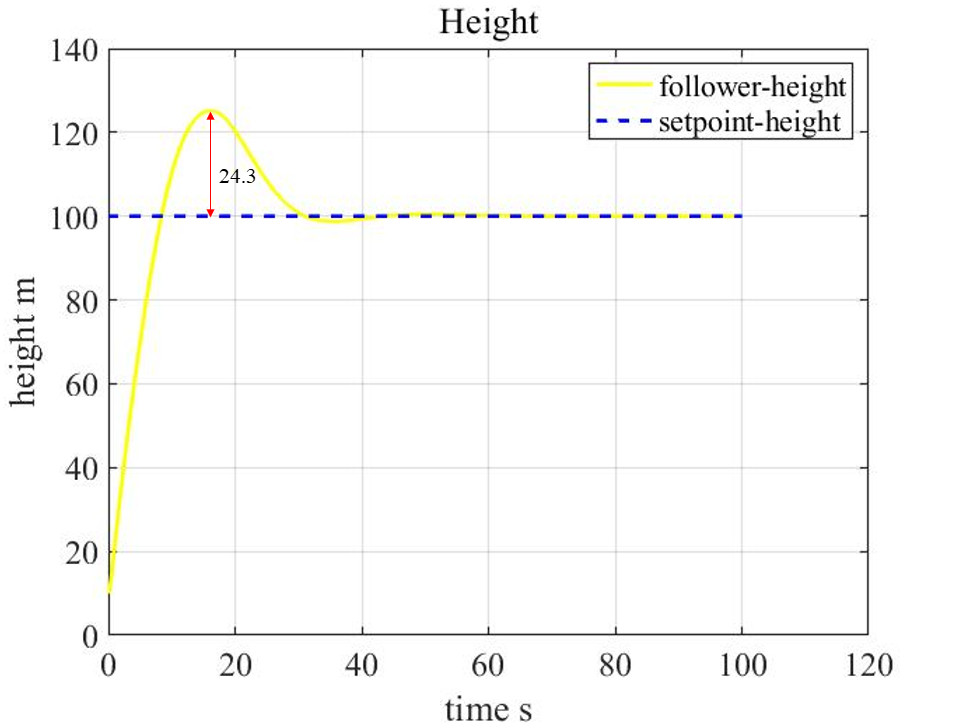
\includegraphics[width=0.85\textwidth]{figures/c5/c5-TECS-height.jpg}
    \caption{竖直平面高度关系}\label{fig:c5-TECS-height}
\end{figure}
\begin{figure}[H]
    \centering
    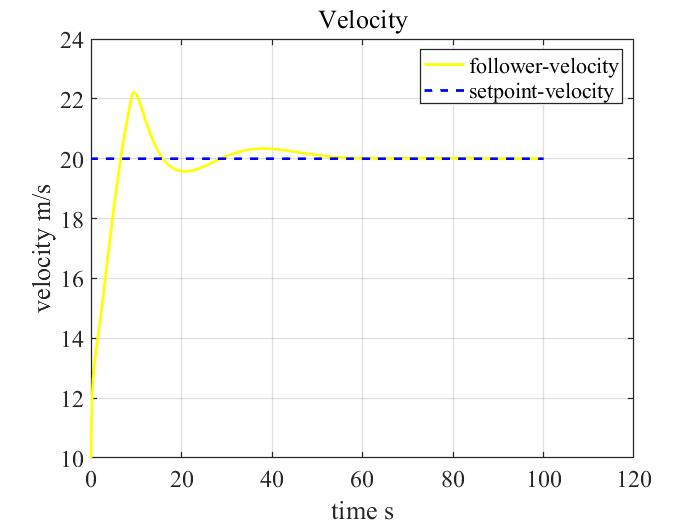
\includegraphics[width=0.85\textwidth]{figures/c5/c5-TECS-vel.jpg}
    \caption{竖直平面速度关系}\label{fig:c5-TECS-vel}
\end{figure}
\begin{figure}[H]
    \centering
    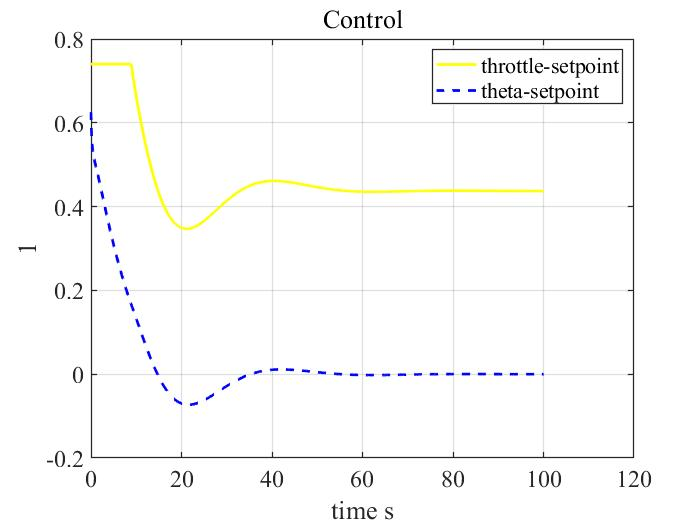
\includegraphics[width=0.85\textwidth]{figures/c5/c5-TECS-control.jpg}
    \caption{竖直平面控制量关系}\label{fig:c5-TECS-control}
\end{figure}
由仿真结果可知,本文所设计的$TECS$控制器可以完成对于期望速度以及期望高度的跟踪,从而达到消除竖直平面内的误差的作用。
\section{基于ROS/Gazebo-PX4的双机编队动力学仿真}
根据第\ref{chap:hardware}章中介绍的ROS-Gazebo仿真环境,进行仿真环境下的双机编队飞行试验。首先利用QGround Control 地面站为领机规划
一条包括起飞以及降落航点在内的一条长直航线。之后先使用地面站将领机1(vehicle 1)
解锁,切换任务模式之后起飞,按照既定航线飞行。等待领机到达第一个
航点之后,再起飞从机2(vehicle 2)
,并切换到外部控制模式,即编队控制的控制逻辑。之后经过一段时间的飞行之后,采集飞行之中的编队误差等数据:最终
编队稳定之后的可视化效果如下:
\begin{figure}[H]
    \centering
    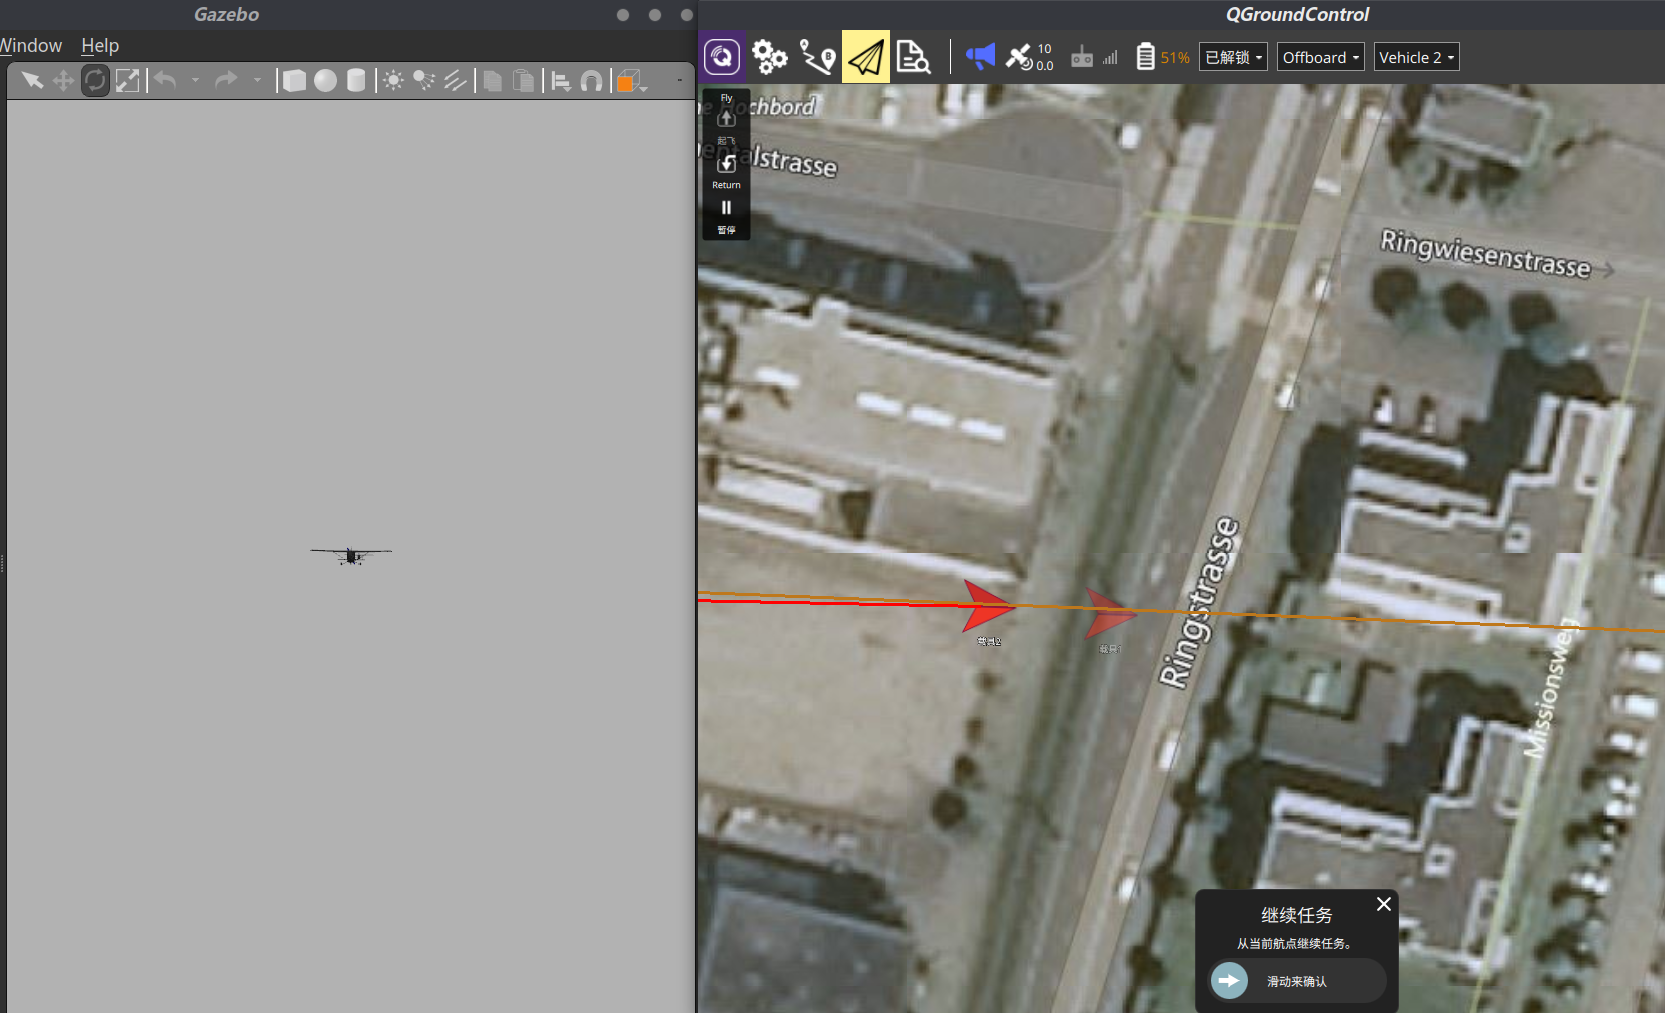
\includegraphics[width=0.85\textwidth]{figures/c5/c5-real-overview}
    \caption{稳定编队之后的编队可视化效果}\label{c5-real-overview}
\end{figure}
在仿真过程中,利用ROS提供的rosbag等数据记录工具,可以进行仿真之中的数据记录与处理:图\ref{c5-real-pos_err_x}-图\ref{c5-real-pos_err_z}分别代表了双机编队位置误差投影在从机坐标系$O_kx_ky_kz_k$中的分量随时间的变化关系;图\ref{c5-real-eta_err}代表从机与领机的速度方向误差随时间变化关系;图\ref{c5-real-vel_err}代表从机与领机的速度大小误差随时间的变化关系。
\begin{figure}[H]
    \centering
    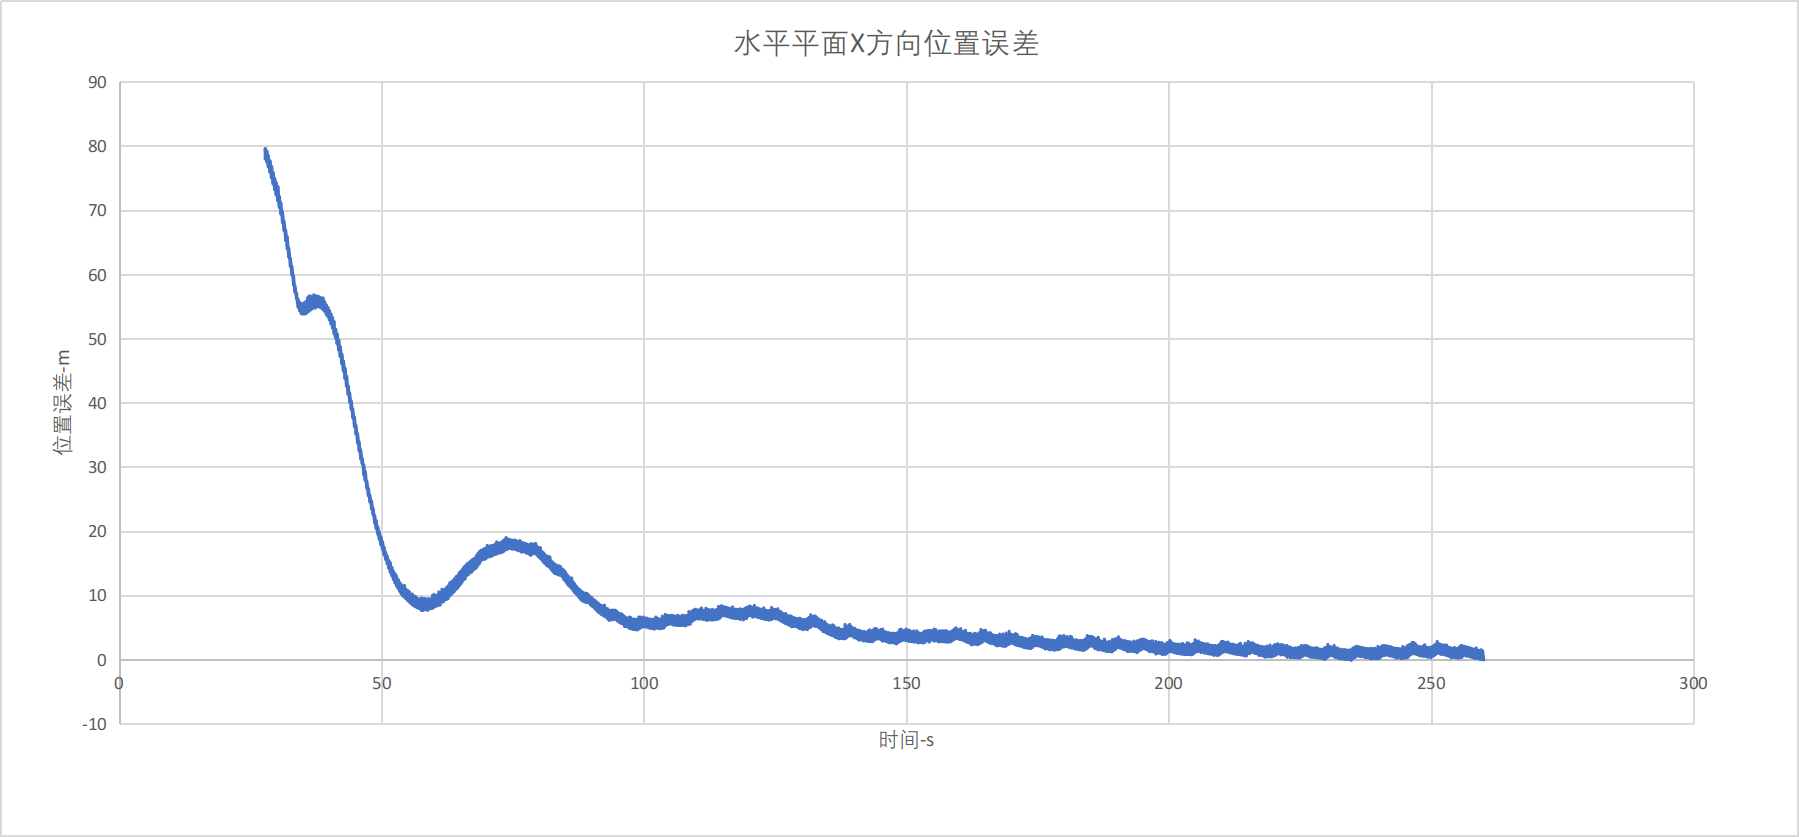
\includegraphics[width=0.85\textwidth]{figures/c5/c5-real-pos_err_x}
    \caption{X通道位置误差}\label{c5-real-pos_err_x}
\end{figure}
\begin{figure}[H]
    \centering
    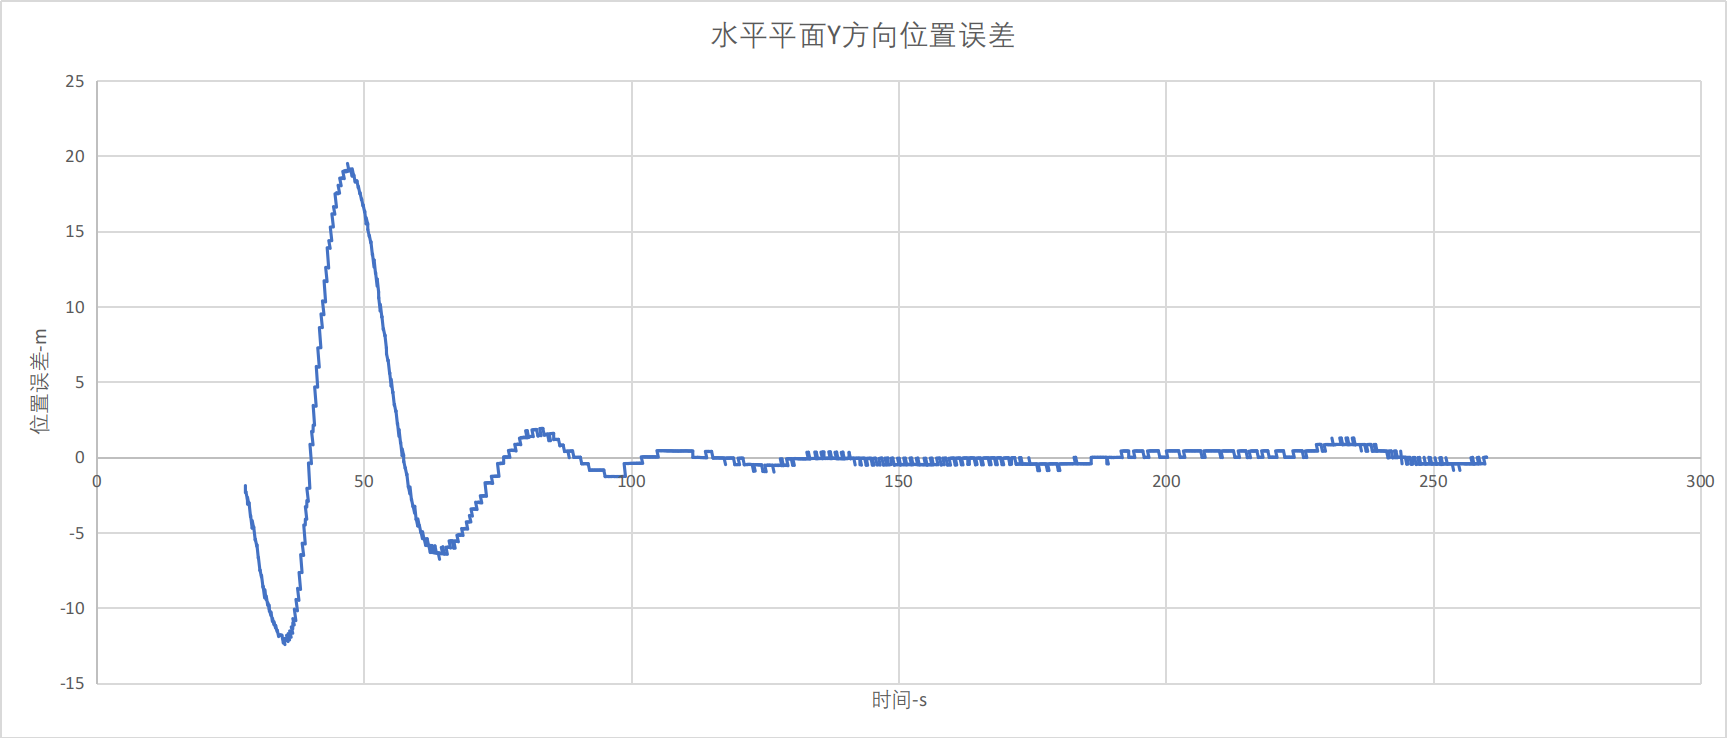
\includegraphics[width=0.85\textwidth]{figures/c5/c5-real-pos_err_y}
    \caption{Y通道位置误差}\label{c5-real-pos_err_y}
\end{figure}
\begin{figure}[H]
    \centering
    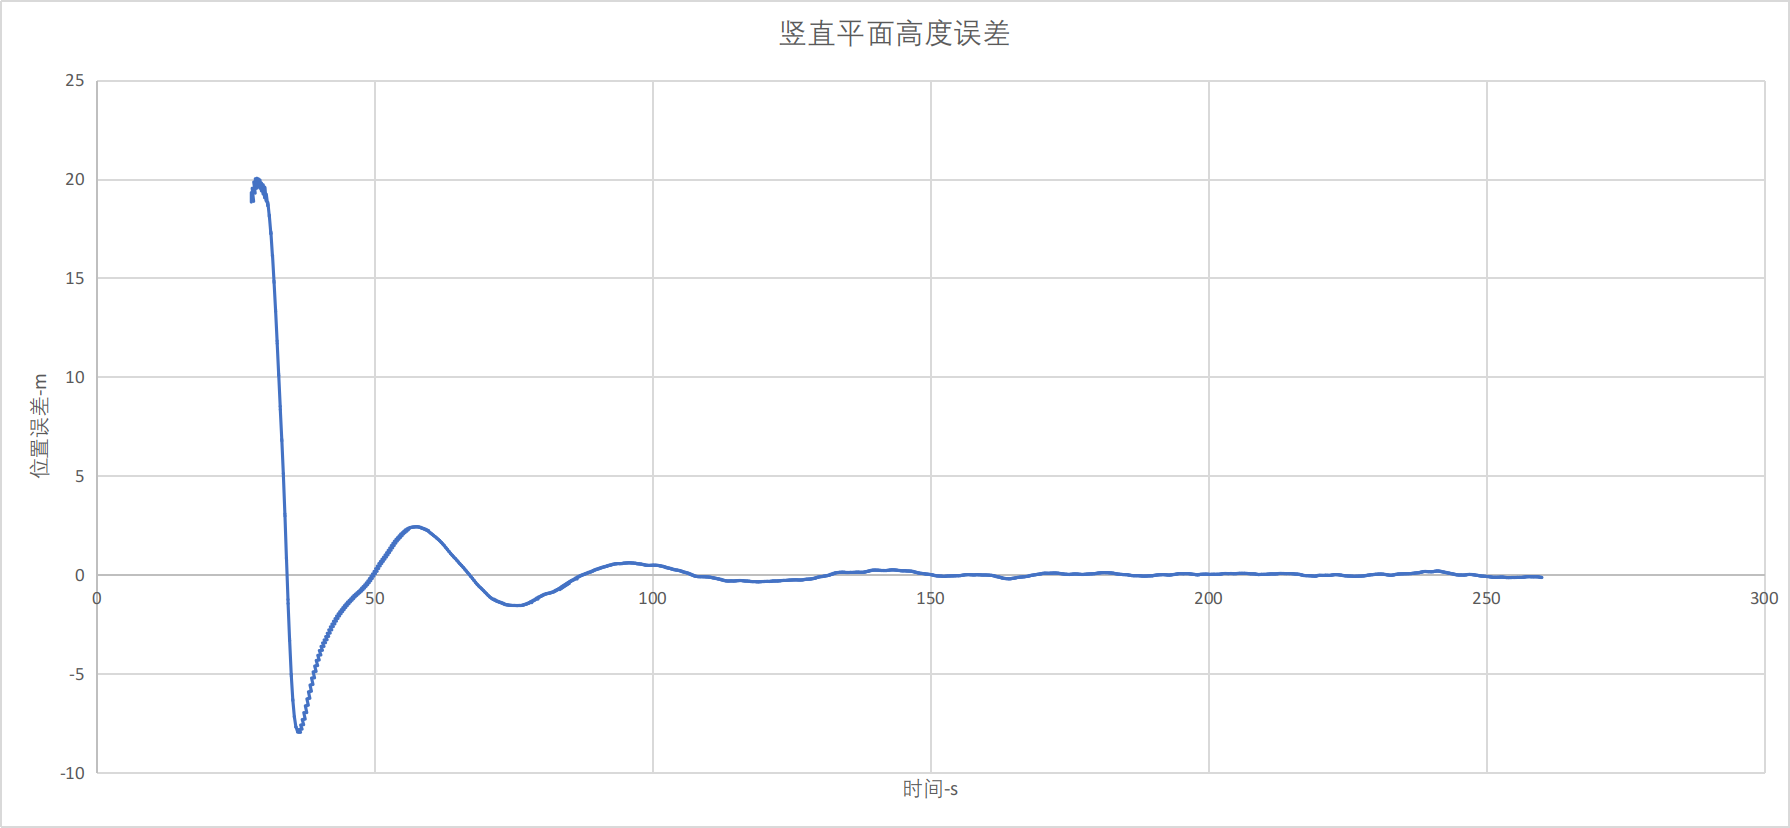
\includegraphics[width=0.85\textwidth]{figures/c5/c5-real-pos_err_z}
    \caption{Z通道位置误差}\label{c5-real-pos_err_z}
\end{figure}
\begin{figure}[H]
    \centering
    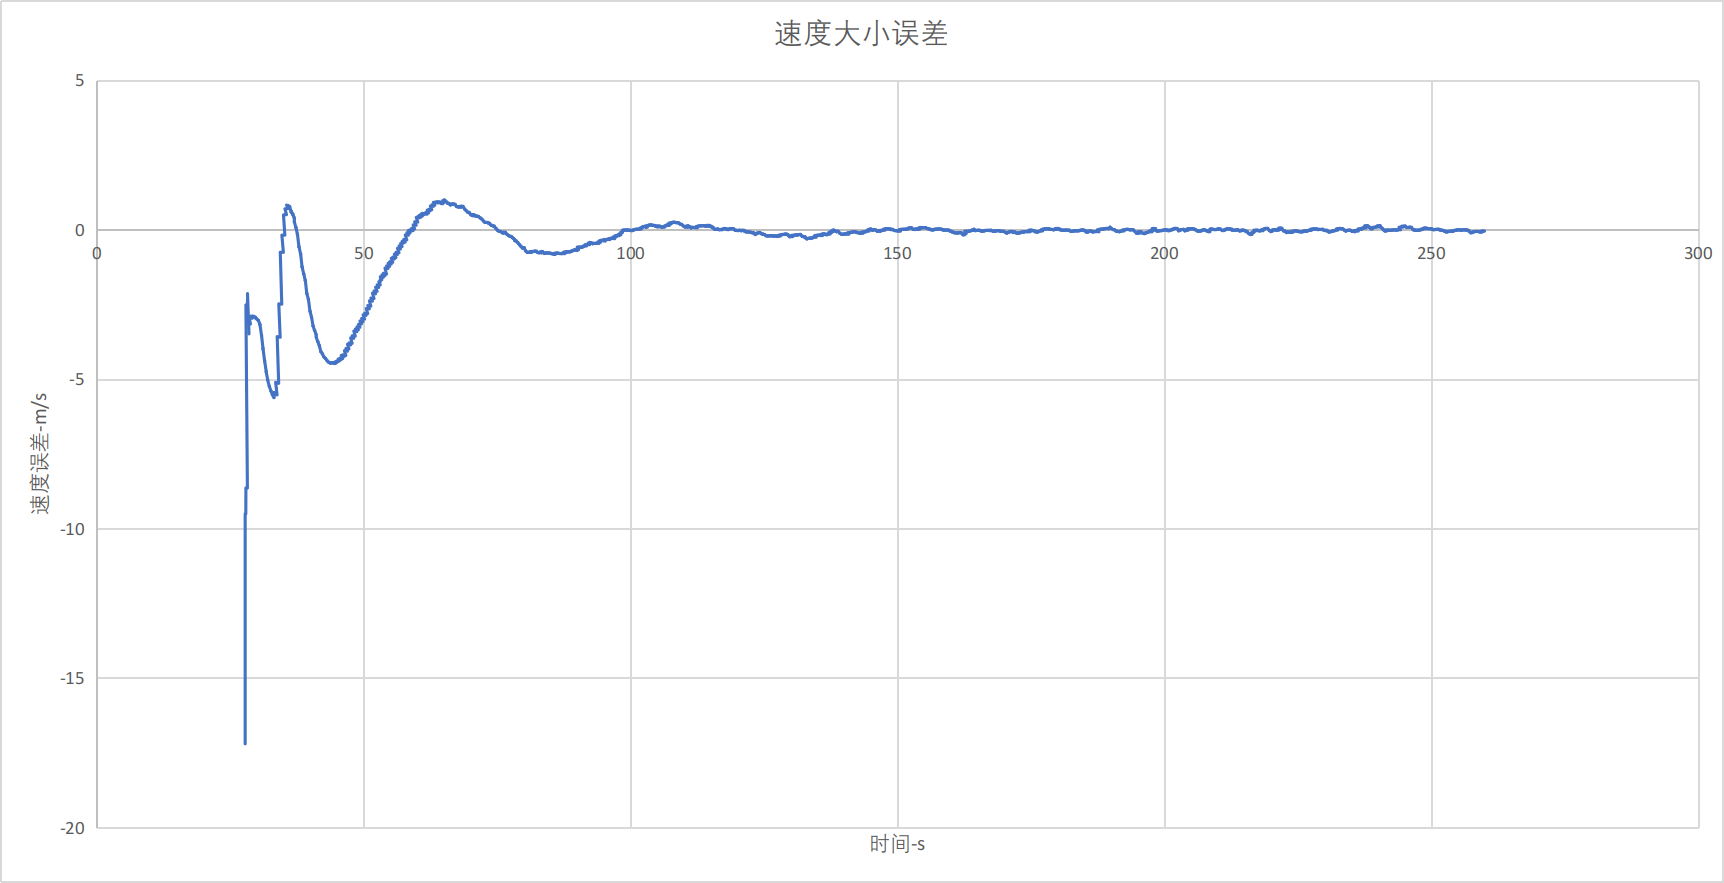
\includegraphics[width=0.85\textwidth]{figures/c5/c5-real-vel_err}
    \caption{领机从机速度大小误差}\label{c5-real-vel_err}
\end{figure}
\begin{figure}[H]
    \centering
    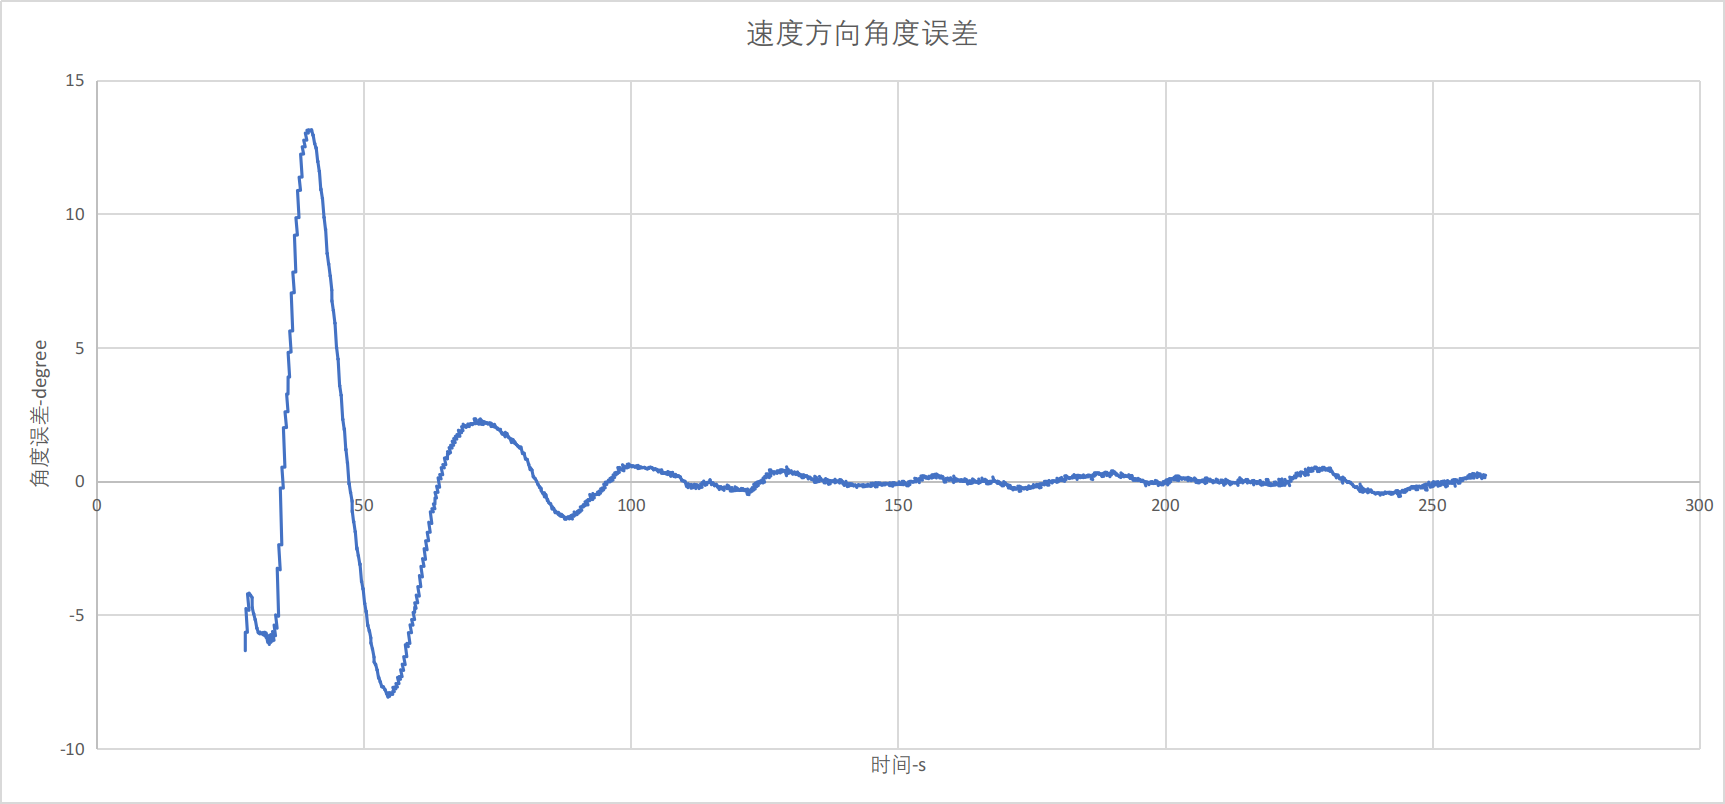
\includegraphics[width=0.85\textwidth]{figures/c5/c5-real-eta_err}
    \caption{领机从机速度方向误差}\label{c5-real-eta_err}
\end{figure}

%\chapter{绪论}
\label{chap:intro}
\section{本文研究的目的和意义}
在未来战场环境中,仅靠单架无人机自主作战无法适应复杂多样的战场环境,而具备协同作战能力的无人机编队能更好地完成任务,与单架无人机相比具有作战效率高、
视野广阔等优势,可实现对目标的全方位立体监视,对地精确攻击。另外,无人机紧密编队可以实现长航任务中无人机的空中加油,对接等任务,如图\ref{fig:c01-meaning}。
编队飞行作为无人机研究领域的热点与难点问题,涉及多项关键技术,例如:队形设计、自主编队、队形保持变换、协调通信等。无人机自主编队控制是实现集群作战的关键技
术。

固定翼无人机以紧密编队的形式飞行,如迁徙的鸟儿一样,可以减少整体的飞行阻力并且减少燃料消耗。整体编队产生的效果将会与精心设计的、具有良好的气动
外形的飞行器相媲美。但是,按照相关文献显示,如果固定翼编队的控制精度无法达到要求精度的10\%,那么最优的减租效果可能会被削减30\%。
 \begin{figure}[H]
  \centering
  \subfigure[无人机编队加受油]{
  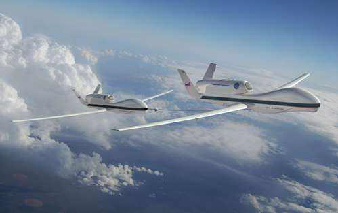
\includegraphics[width=0.45\textwidth]{figures/c1/c01-meaning-1.png} 
}
  \subfigure[无人机编队巡航]{
  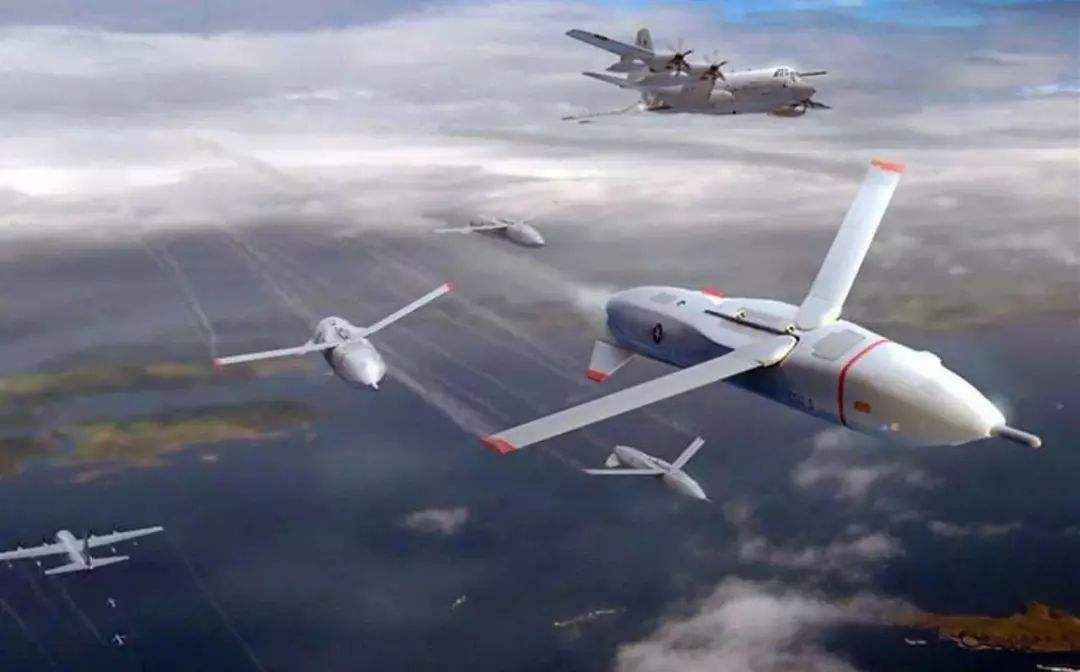
\includegraphics[width=0.45\textwidth]{figures/c1/c01-meaning-2.jpeg}
}
  \caption{无人机编队应用场景}
  \label{fig:c01-meaning}
  \end{figure}
%\upcite{Takahashi1996Structure,Xia2002Analysis,Jiang1989,Mao2000Motion,Feng1998}%这个是文献引用上标
\section{国内外研究现状及发展趋势}
%\label{sec:***} 可标注label
现如今的无人机自动驾驶仪的结构由导航模块、位置控制控制模块(外环)以及姿态控制模块(内环)组成;导航模块产生期望位置,位置控制模块由期望位置产生
期望姿态角,姿态控制模块由期望姿态角产生最终的伺服系统的控制量。现如今的低成本无人机所使用的传感器硬件精度比较低,均为消费级别,如果不考虑传感
器的精度问题而设计控制方案,很可能导致整体编队的控制精度下降。现如今已经存在的大部分编队控制算法均为考虑飞机的质点运动学以及质点动力学条件下提
出的导航方法,最终产生的飞行器的控制量为无人机航迹坐标系下的加速度期望值以及飞机的航向角的期望角速度。按照飞机的控制方式,需要将航迹坐标系下的
期望控制量转到机体系之下,但是飞机自动驾驶仪并不能接受加速度控制量,尤其是飞机机体$O_bx_b$轴方向,无人机推力、阻力以及重力沿机体方向的推力并非是代数关
系,不能直接由期望加速度得到期望推力;无人机姿态驾驶仪常使用协调转弯模型作为内环角度环的控制基础,不能直接响应所给出的偏航角速度的期望值。另外由于低成
本无人机的惯性原件的精度问题导致无人机不能使用测量的加速度信息作为反馈,两种原因导致以加速度
为最终控制量对于低成本无人机编队的方法控制精度不足。

%TODO:此处的引用存疑
目前的编队控制已经提出多种方案,例如:基于距离的编队控制策略、人工势场法,基于距离的编队控制,基于行为的编队控制,基于虚拟结构的编队控制,基于虚
拟领机的编队控制等。其中,基于距离编队中的领从模式因其原理简单而得到广泛应用。本文正是基于领从策略(leader-follower method)设计的编队控制器。
\section{本文的技术方案}
%\label{sec:***} 可标注label
首先建立无人机编队的领机与从机相对运动模型,描述领机从机在三维空间之内的运动规律。其次按照编队的控制目标设计编队控制器的误差输入量,并按照无人机
的内环的输入量,设计编队控制的数学形式。之后再完成无人机质点模型下的编队控制率仿真,完善编队所设计编队控制器的结构。之后,利用ROS/Gazebo等仿真包搭建
无人机编队动力学仿真环境,测试编队控制再考虑自动驾驶仪内环以及无人机的动力学模型之后的编队控制表现。最后,进行实际飞行的测试:记录编队控制的实际动态特性
稳态特性、飞行编队的抗干扰能力、以及编队的能源节约情况。
\section{本文的组织结构}
本文之后的部分将如下组织:第二章建立无人机编队的动力学模型;第三章设计编队控制器数学形式;第四章介绍无人机编队整体控制逻辑、仿真环境以及硬件选型
;第五章控制器仿真以及实际飞行实验结果分析;第六章为结论。


% 结论:在结论相应的 TeX 文件处进行结论部分的撰写
%%
% The BIThesis Template for Bachelor Graduation Thesis
%
% 北京理工大学毕业设计(论文)结论 —— 使用 XeLaTeX 编译
%
% Copyright 2020 Spencer Woo
%
% This work may be distributed and/or modified under the
% conditions of the LaTeX Project Public License, either version 1.3
% of this license or (at your option) any later version.
% The latest version of this license is in
%   http://www.latex-project.org/lppl.txt
% and version 1.3 or later is part of all distributions of LaTeX
% version 2005/12/01 or later.
%
% This work has the LPPL maintenance status `maintained'.
%
% The Current Maintainer of this work is Spencer Woo.
%
% Compile with: xelatex -> biber -> xelatex -> xelatex

\addcontentsline{toc}{chapter}{结~~~~论}
\chapter*{\vskip 10bp\textmd{结~~~~论} \vskip -6bp}

% 在结论部分的子标题不需要序号,加上 * 即可(一个例子如下)
% \section*{结论段落标题}

% 这里插入一个参考文献,仅作参考
本文结论……。\cite{dengImageNetLargescaleHierarchical2010}

\textcolor{blue}{结论作为毕业设计(论文)正文的最后部分单独排写,但不加章号。结论是对整个论文主要结果的总结。在结论中应明确指出本研究的创新点,对其应用前景和社会、经济价值等加以预测和评价,并指出今后进一步在本研究方向进行研究工作的展望与设想。结论部分的撰写应简明扼要,突出创新性。阅后删除此段。}

\textcolor{blue}{结论正文样式与文章正文相同:宋体、小四;行距:22 磅;间距段前段后均为 0 行。阅后删除此段。}

% 参考文献:如无特殊需要,参考文献相应的 TeX 文件无需改动,添加参考文献请使用 BibTeX 的格式
%   添加至 misc/ref.bib 中,并在正文的相应位置使用 \cite{xxx} 的格式引用参考文献
%%
% The BIThesis Template for Bachelor Graduation Thesis
%
% 北京理工大学毕业设计(论文)参考文献 —— 使用 XeLaTeX 编译
%
% Copyright 2020 Spencer Woo
%
% This work may be distributed and/or modified under the
% conditions of the LaTeX Project Public License, either version 1.3
% of this license or (at your option) any later version.
% The latest version of this license is in
%   http://www.latex-project.org/lppl.txt
% and version 1.3 or later is part of all distributions of LaTeX
% version 2005/12/01 or later.
%
% This work has the LPPL maintenance status `maintained'.
%
% The Current Maintainer of this work is Spencer Woo.
%
% Compile with: xelatex -> biber -> xelatex -> xelatex
%
% 如无特殊需要,本页面无需更改

% 参考文献开始
\chapter*{\vskip 10bp \textmd{参考文献} \vskip -6bp}
\addcontentsline{toc}{chapter}{参考文献}

% 设置参考文献字号为 5 号
\renewcommand*{\bibfont}{\zihao{5}}
% 设置参考文献各个项目之间的垂直距离为 0
\setlength{\bibitemsep}{0ex}
\setlength{\bibnamesep}{0ex}
\setlength{\bibinitsep}{0ex}
% 设置单倍行距
\renewcommand{\baselinestretch}{1.2}
% 设置参考文献顺序标签 `[1]` 与文献内容 `作者. 文献标题...` 的间距
\setlength{\biblabelsep}{0.5mm}
% 设置参考文献后文缩进为 0(与 Word 模板保持一致)
\renewcommand{\itemcmd}{
  \addvspace{\bibitemsep} % 恢复 \bibitemsep 的作用
  \mkgbnumlabel{\printfield{labelnumber}}
  \hspace{\biblabelsep}}

% 删除默认的「参考文献 / Reference」标题,使用上面定义的 section 标题
\printbibliography[heading=none]

% 附录:在附录相应的 TeX 文件处进行附录部分的撰写
%%
% The BIThesis Template for Bachelor Graduation Thesis
%
% 北京理工大学毕业设计(论文)附录 —— 使用 XeLaTeX 编译
%
% Copyright 2020 Spencer Woo
%
% This work may be distributed and/or modified under the
% conditions of the LaTeX Project Public License, either version 1.3
% of this license or (at your option) any later version.
% The latest version of this license is in
%   http://www.latex-project.org/lppl.txt
% and version 1.3 or later is part of all distributions of LaTeX
% version 2005/12/01 or later.
%
% This work has the LPPL maintenance status `maintained'.
%
% The Current Maintainer of this work is Spencer Woo.
%
% Compile with: xelatex -> biber -> xelatex -> xelatex

\addcontentsline{toc}{chapter}{附~~~~录}
\chapter*{\vskip 10bp \textmd{附~~~~录} \vskip -6bp}

附录相关内容…

\textcolor{blue}{附录是毕业设计(论文)主体的补充项目,为了体现整篇文章的完整性,写入正文又可能有损于论文的条理性、逻辑性和精炼性,这些材料可以写入附录段,但对于每一篇文章并不是必须的。附录依次用大写正体英文字母 A、B、C……编序号,如附录 A、附录 B。阅后删除此段。}

\textcolor{blue}{附录正文样式与文章正文相同:宋体、小四;行距:22 磅;间距段前段后均为 0 行。阅后删除此段。}

% 致谢:在致谢相应的 TeX 文件处进行致谢部分的撰写
%%
% The BIThesis Template for Bachelor Graduation Thesis
%
% 北京理工大学毕业设计(论文)致谢 —— 使用 XeLaTeX 编译
%
% Copyright 2020 Spencer Woo
%
% This work may be distributed and/or modified under the
% conditions of the LaTeX Project Public License, either version 1.3
% of this license or (at your option) any later version.
% The latest version of this license is in
%   http://www.latex-project.org/lppl.txt
% and version 1.3 or later is part of all distributions of LaTeX
% version 2005/12/01 or later.
%
% This work has the LPPL maintenance status `maintained'.
%
% The Current Maintainer of this work is Spencer Woo.
%
% Compile with: xelatex -> biber -> xelatex -> xelatex

\chapter*{\vskip 10bp \textmd{致~~~~谢} \vskip -6bp}
\addcontentsline{toc}{chapter}{致~~~~谢}

正值本文完成之际,首先我想感谢母校北京理工大学能够给我这个机会让我可以完成毕业设计,为我的本科学习画上一个圆满的句号。

其次我想感谢的便是我的指导老师王佳楠老师。从初有固定翼编队控制的方向,到实验室固定翼项目组成立,再到本次毕业设计的完成,王老师以他
严谨的治学风格,高昂的学术热情,精益求精的工作作风,无论在学术之路还是人生发展方向都给了我莫大的感染与激励!无论是资金还是学习机会,
王老师总是尽力提供给我。在这些宝贵的学习机会之中,我对固定翼的控制的理解逐渐加深。
固定翼编队的项目,跌跌撞撞做了一年有余,正因为有成功时王老师给予我的赞扬,失利时给予我的鼓励与指导,此项目才得以到达今日。
古人云:“一日为师终生为父”,笔者认为莫过如此!

系统与仿真实验室给了我一个如同家一样的地方,实验室中许多老师,例如丁艳老师,王春彦老师,王丹丹老师都曾经给过我许多帮助,并让我得以
实现心中所想,感谢系统与仿真实验室的一代代的建设者!在这之后,我要感谢亲自指导我的苏 劭署学长,是他将ROS-Gazebo这一
套系统第一次应用到了固定翼飞行平台之上;戚煜华、江佳奇师兄帮我解答了环境配置的相关问题并为我介绍了许多志同道合的人士;周正阳学长帮助我
解答了许多硬件问题以及通信的相关问题;陈亚东以及丁祥军学长解答了一系列的飞行器导航与制导的相关问题,在此一并致谢!固定翼小组在
成立之时,每个成员都为固定翼的控制贡献出了自己的力量与智慧;他们分别是孙浩、郑志强、赵亚明、罗正昕、鲁冰洁、刘哲伟同学以及2017
届学弟查家军、姜浩舸、张艺弘以及胡牧天学弟,感谢你们的并肩协力!

本项目还得到了国内阿木社区王根等几位前辈在硬件上的指导与帮助; 太原理工大学航模队杨明老师和他的团队以及荷兰代尔夫特理工大学王曦漫博士和他的团队帮
助我解决了固定翼多机编队仿真的环境问题,在此感谢上述前辈们的悉心指导!

此外,在前期的固定翼外场实验中,我的老搭档张智铎、范铮铮同学以及2015级航模队队长刘天学长、同届飞手教练孙黎明学长为在烈日酷暑下为此
项目实地实验,感谢你们的鼎力相助!



\end{document}
